% Contents from body/page-438.tex.
\BookMark{0}{Appendix A  Intersection Theory}{p-438}
\ChapterSheet{438}{424}{}{%
\vspace*{22pt}
\noindent{\large\bfseries Appendix A}\par\vspace{3pt}
\hrule
\vspace{6pt}
\noindent{\Large\bfseries Intersection Theory}\par
\vspace{161pt}
\noindent In this appendix we will outline the generalization of intersection theory and the Riemann--Roch theorem to nonsingular projective varieties of any dimension. To motivate the discussion, let us look at the case of curves and surfaces, and then see what needs to be generalized. For a divisor $D$ on a curve $X$, leaving out the contribution of Serre duality, we can write the Riemann--Roch theorem (IV, \Goto{result-IV-1.3}{1.3}) as
\[
\chi(\mathcal L(D))=\deg D+1-g,
\]
where $\chi$ is the Euler characteristic (III, Ex.~\Goto{ex-III-5.1}{5.1}). On a surface, we can write the Riemann--Roch theorem (V, \Goto{result-V-1.6}{1.6}) as
\[
\chi(\mathcal L(D))=\frac12 D\cdot(D-K)+1+p_a.
\]

In each case, on the left-hand side we have something involving cohomology groups of the sheaf $\mathcal L(D)$, while on the right-hand side we have some numerical data involving the divisor $D$, the canonical divisor $K$, and some invariants of the variety $X$. Of course the ultimate aim of a Riemann--Roch type theorem is to compute the dimension of the linear system $|D|$ or of $|nD|$ for large $n$ (II, Ex.~\Goto{ex-II-7.6}{7.6}). This is achieved by combining a formula for $\chi(\mathcal L(D))$ with some vanishing theorems for $H^i(X,\mathcal L(D))$ for $i>0$, such as the theorems of Serre (III, \Goto{result-III-5.2}{5.2}) or Kodaira (III, \Goto{result-III-7.15}{7.15}).

We will now generalize these results so as to give an expression for $\chi(\mathcal L(D))$ on a nonsingular projective variety $X$ of any dimension. And while we are at it, with no extra effort we get a formula for $\chi(\mathcal E)$, where $\mathcal E$ is any coherent locally free sheaf.

To generalize the right-hand side, we need an intersection theory on $X$. The intersection of two divisors, for example, will not be a number, but a
}
% Contents from body/page-439.tex.
\BookMark{1}{A.1  Intersection Theory}{sec-A-1}
\ChapterSheet{439}{425}{\Goto{sec-A-1}{1\quad Intersection Theory}}{%
\emph{cycle} of codimension $2$, which is a linear combination of subvarieties of codimension $2$. So we will introduce the language of cycles and rational equivalence (which generalizes the linear equivalence of divisors), in order to set up our intersection theory.

We also need to generalize the correspondence between the invertible sheaf $\mathcal L(D)$ and the divisor $D$. This is accomplished by the theory of Chern classes: to each locally free sheaf $\mathcal E$ of rank $r$, we associate Chern classes $c_1(\mathcal E),\ldots,c_r(\mathcal E)$, where $c_i(\mathcal E)$ is a cycle of codimension $i$, defined up to rational equivalence.

As for invariants of the variety $X$, the canonical class $K$ and the arithmetic genus $p_a$ are not enough in general, so we use all the Chern classes of the tangent sheaf of $X$ as well.

Then the generalized Riemann--Roch theorem will give a formula for $\chi(\mathcal E)$ in terms of certain intersection numbers of the Chern classes of $\mathcal E$ and of the tangent sheaf of $X$.

\bigskip
\noindent\hypertarget{sec-A-1}{}{\large\bfseries 1\quad Intersection Theory}\par
\medskip
\noindent The intersection theory on a surface (V, \Goto{result-V-1.1}{1.1}) can be summarized by saying that there is a unique symmetric bilinear pairing $\operatorname{Pic} X\times\operatorname{Pic} X\to\mathbb Z$, which is \emph{normalized} by requiring that for any two irreducible nonsingular curves $C,D$ meeting transversally, $C\cdot D$ is just the number of intersection points of $C$ and $D$. Our main tool in proving this theorem was Bertini's theorem, which allowed us to move any two divisors in their linear equivalence class, so that they became differences of irreducible nonsingular curves meeting transversally.

\smallskip
In higher dimensions, the situation is considerably more complicated. The corresponding moving lemma is weaker, so we need a stronger normalization requirement. It turns out that the most convenient way to develop intersection theory is to do it for all varieties at once, and include some functorial mappings $f_*$ and $f^*$ associated to a morphism $f\colon X\to X'$ as part of the structure.

Let $X$ be any variety over $k$. A \emph{cycle of codimension $r$} on $X$ is an element of the free abelian group generated by the closed irreducible subvarieties of $X$ of codimension $r$. So we write a cycle as $Y=\sum n_iY_i$ where the $Y_i$ are subvarieties, and $n_i\in\mathbb Z$. Sometimes it is useful to speak of the cycle associated to a closed subscheme. If $Z$ is a closed subscheme of codimension $r$, let $Y_1,\ldots,Y_t$ be those irreducible components of $Z$ which have codimension $r$, and define the \emph{cycle associated} to $Z$ to be $\sum n_iY_i$, where $n_i$ is the length of the local ring $\mathcal O_{y_i,Z}$ of the generic point $y_i$ of $Y_i$ on $Z$.

Let $f\colon X\to X'$ be a morphism of varieties, and let $Y$ be a subvariety of $X$. If $\dim f(Y)<\dim Y$, we set $f_*(Y)=0$. If $\dim f(Y)=\dim Y$, then the function field $K(Y)$ is a finite extension field of $K(f(Y))$, and we set
\[
f_*(Y)=[K(Y):K(f(Y))]\cdot\overline{f(Y)}.
\]
}
% Contents from body/page-440.tex.
\ChapterSheet{440}{426}{\Goto{p-438}{Appendix A\quad Intersection Theory}}{%
Extending by linearity defines a homomorphism $f_*$ of the group of cycles on $X$ to the group of cycles on $X'$.

\smallskip
Now we come to the definition of rational equivalence. For any subvariety $V$ of $X$, let $f\colon\widetilde V\to V$ be the normalization of $V$. Then $\widetilde V$ satisfies the condition \Goto{cond-II-6-star}{($*$)} of (II, \Goto{sec-II-6}{\S6}), so we can talk about Weil divisors and linear equivalence on $\widetilde V$. Whenever $D$ and $D'$ are linearly equivalent Weil divisors on $\widetilde V$, we say that $f_*D$ and $f_*D'$ are \emph{rationally equivalent} as cycles on $X$. Then we define \emph{rational equivalence} of cycles on $X$ in general by dividing out by the group generated by all such $f_*D\sim f_*D'$ for all subvarieties $V$, and all linearly equivalent Weil divisors $D,D'$ on $\widetilde V$. In particular, if $X$ itself is normal, then rational equivalence for cycles of codimension $1$ coincides with linear equivalence of Weil divisors.

For each $r$ we let $A^r(X)$ be the group of cycles of codimension $r$ on $X$ modulo rational equivalence. We denote by $A(X)$ the graded group $\bigoplus_{r=0}^n A^r(X)$, where $n=\dim X$. Note that $A^0(X)=\mathbb Z$, and that $A^r(X)=0$ for $r>\dim X$. Note also that if $X$ is complete there is a natural group homomorphism, the \emph{degree}, from $A^n(X)$ to $\mathbb Z$, defined by $\deg(\sum n_iP_i)=\sum n_i$, where the $P_i$ are points. This is well-defined on rational equivalence classes because of (II, \Goto{result-II-6.10}{6.10}).

\smallskip
An intersection theory on a given class of varieties $\mathfrak B$ consists of giving a pairing $A^r(X)\times A^s(X)\to A^{r+s}(X)$ for each $r,s$, and for each $X\in\mathfrak B$, satisfying the axioms listed below. If $Y\in A^r(X)$ and $Z\in A^s(X)$ we denote the intersection cycle class by $Y\cdot Z$.

Before stating the axioms, for any morphism $f\colon X\to X'$ of varieties in $\mathfrak B$, we assume that $X\times X'$ is also in $\mathfrak B$, and we define a homomorphism $f^*\colon A(X')\to A(X)$ as follows. For a subvariety $Y'\subseteq X'$ we define
\EditionText{%
\[
f^*([Y'])=\gamma_f^!\bigl(p_2^*[Y']\bigr),
\]
where $p_1,p_2$ are the projections of $X\times X'$, and $\gamma_f\colon X\hookrightarrow X\times X'$ is the graph embedding. For nonsingular $X,X'$, $\gamma_f^!$ is the Gysin pullback for the regular embedding $\gamma_f$. This is the refined intersection of the graph and $p_2^{-1}(Y')$ on their intersection, carried to $X$ by the restriction of $p_1$.%
}

This data is now subject to the following requirements.

\hypertarget{axiom-A-A1}{}A1. The intersection pairing makes $A(X)$ into a commutative associative graded ring with identity, for every $X\in\mathfrak B$. It is called the \emph{Chow ring} of $X$.

\hypertarget{axiom-A-A2}{}A2. For any morphism $f\colon X\to X'$ of varieties in $\mathfrak B$, $f^*\colon A(X')\to A(X)$ is a ring homomorphism. If $g\colon X'\to X''$ is another morphism, then $f^*\circ g^*=(g\circ f)^*$.

\hypertarget{axiom-A-A3}{}A3. For any proper morphism $f\colon X\to X'$ of varieties in $\mathfrak B$, $f_*\colon A(X)\to A(X')$ is a homomorphism of graded groups (which shifts degrees). If $g\colon X'\to X''$ is another \EditionText{proper }morphism, then $g_*\circ f_*=(g\circ f)_*$.

\hypertarget{axiom-A-A4}{}A4. \emph{Projection formula.} If $f\colon X\to X'$ is a proper morphism, if $x\in A(X)$ and $y\in A(X')$, then
\[
f_*(x\cdot f^*y)=f_*(x)\cdot y.
\]
}
% Contents from body/page-441.tex.
\ChapterSheet{441}{427}{\Goto{sec-A-1}{1\quad Intersection Theory}}{%
\indent\hypertarget{axiom-A-A5}{}A5. \emph{Reduction to the diagonal.} If $Y$ and $Z$ are cycles on $X$, and if $\Delta\colon X\to X\times X$ is the diagonal morphism, then
\[
Y\cdot Z=\Delta^*(Y\times Z).
\]

\hypertarget{axiom-A-A6}{}A6. \emph{Local nature.} If $Y$ and $Z$ are subvarieties of $X$ which \emph{intersect properly} (meaning that every irreducible component of $Y\cap Z$ has codimension equal to $\operatorname{codim}Y+\operatorname{codim}Z$), then we can write
\[
Y\cdot Z=\sum i(Y,Z;W_j)W_j,
\]
where the sum runs over the irreducible components $W_j$ of $Y\cap Z$, and where the integer $i(Y,Z;W_j)$ depends only on a neighborhood of the generic point of $W_j$ on $X$. We call $i(Y,Z;W_j)$ the \emph{local intersection multiplicity} of $Y$ and $Z$ along $W_j$.

\hypertarget{axiom-A-A7}{}A7. \emph{Normalization.} If $Y$ is a subvariety of $X$, and $Z$ is an effective Cartier divisor meeting $Y$ properly, then $Y\cdot Z$ is just the cycle associated to the Cartier divisor $Y\cap Z$ on $Y$, which is defined by restricting the local equation of $Z$ to $Y$. (This implies in particular that transversal intersections of nonsingular subvarieties have multiplicity $1$.)

\medskip
\noindent\hypertarget{result-A-1.1}{}\textbf{Theorem 1.1.} \emph{Let $\mathfrak B$ be the class of nonsingular quasi-projective varieties over a fixed algebraically closed field $k$. Then there is a unique intersection theory for cycles modulo rational equivalence on the varieties $X\in\mathfrak B$ which satisfies the axioms \Goto{axiom-A-A1}{A1}--\Goto{axiom-A-A7}{A7} above.}

\medskip
There are two main ingredients in the proof of this theorem. One is the correct definition of the local intersection multiplicities; the other is Chow's moving lemma. There are several ways of defining intersection multiplicity. We just mention Serre's definition, which is historically most recent, but has the advantage of being compact. If $Y$ and $Z$ intersect properly, and if $W$ is an irreducible component of $Y\cap Z$, we define
\[
i(Y,Z;W)=\sum(-1)^i\operatorname{length}\operatorname{Tor}^A_i(A/\mathfrak a,A/\mathfrak b)
\]
where $A$ is the local ring $\mathcal O_{w,X}$ of the generic point of $W$ on $X$, and $\mathfrak a$ and $\mathfrak b$ are the ideals of $Y$ and $Z$ in $A$. Serre \Goto{bib-481-11}{[11]} shows that this is a nonnegative integer, and that it has the required properties. Note in particular that the naive definition, taking the length of $A/(\mathfrak a+\mathfrak b)=A/\mathfrak a\otimes A/\mathfrak b$, modeled after the case of curves on a surface (V, \Goto{result-V-1.4}{1.4}) does not work \Goto{result-A-1.1.1}{(1.1.1)}.

The other ingredient is \emph{Chow's moving lemma}, which says that if $Y,Z$ are cycles on a nonsingular quasi-projective variety $X$, then there is a cycle $Z'$, rationally equivalent to $Z$, such that $Y$ and $Z'$ intersect properly. Furthermore, if $Z''$ is another such, then $Y\cdot Z'$ and $Y\cdot Z''$ are rationally equivalent. There are proofs of this moving lemma by Chevalley \Goto{bib-chevalley-2}{[2]} and Roberts \Goto{bib-roberts-1}{[1]}.

The uniqueness of the intersection theory is proved as follows: given cycles $Y,Z$ on $X$, by the moving lemma we may assume they intersect properly.
}
% Contents from body/page-442.tex.
\BookMark{1}{A.2  Properties of the Chow Ring}{sec-A-2}
\ChapterSheet{442}{428}{\Goto{p-438}{Appendix A\quad Intersection Theory}}{%
Then using the reduction to the diagonal \Goto{axiom-A-A5}{(A5)} we reduce to the case of computing $\Delta\cdot(Y\times Z)$ on $X\times X$. This has the advantage that $\Delta$ is a local complete intersection. Since the intersection multiplicity is local \Goto{axiom-A-A6}{(A6)} we reduce to the case where one of the cycles is a complete intersection of Cartier divisors, and then repeated application of the normalization \Goto{axiom-A-A7}{(A7)} gives the uniqueness.

Some general references for intersection theory are Weil \Goto{bib-483-4}{[1]}, Chevalley \Goto{bib-chevalley-2}{[2]}, Samuel \Goto{bib-samuel-1}{[1]}, and Serre \Goto{bib-481-11}{[11]}. For discussion of some other equivalence relations on cycles, and attempts to calculate the groups $A^i(X)$, see Hartshorne \Goto{bib-hartshorne-6}{[6]}.

\medskip
\noindent\hypertarget{result-A-1.1.1}{}\textbf{Example 1.1.1.} To see why the higher Tor's are necessary, let $Y$ be the union of two planes in $\AffSpace{4}$ meeting at a point, so the ideal of $Y$ is $(x,y)\cap(z,w)=(xz,xw,yz,yw)$. Let $Z$ be the plane $(x-z,y-w)$. Since $Z$ meets each component of $Y$ in one point $P$, we have $i(Y,Z;P)=2$ by linearity. However, if we naively take $A/(\mathfrak a+\mathfrak b)$ where $\mathfrak a,\mathfrak b$ are the ideals of $Y$ and $Z$, we get
\[
k[x,y,z,w]/(xz,xw,yz,yw,x-z,y-w)\cong k[x,y]/(x^2,xy,y^2),
\]
which has length $3$.

\medskip
\noindent\hypertarget{result-A-1.1.2}{}\textbf{Example 1.1.2.} We cannot expect to have an intersection theory like the one of the theorem on singular varieties. For example, suppose there was an intersection theory on the quadric cone $Q$ given by $xy=z^2$ in $\Proj^3$. Let $L$ be the ruling $x=z=0$, and $M$ the ruling $y=z=0$. Then $2M$ is linearly equivalent to a hyperplane section, which could be taken to be a conic $C$ on $Q$ which meets $L,M$ each transversally in one point. So
\EditionText{%
\[
1=\deg(L\cdot C)=\deg(L\cdot(2M))=2\deg(L\cdot M).
\]
This contradicts the integrality of $\deg(L\cdot M)$.%
}

\bigskip
\noindent\hypertarget{sec-A-2}{}{\large\bfseries 2\quad Properties of the Chow Ring}\par
\medskip
\noindent For any nonsingular quasi-projective variety $X$ we now consider the Chow ring $A(X)$, and list some of its properties. See Chevalley \Goto{bib-chevalley-2}{[2]} for proofs.

\hypertarget{axiom-A-A8}{}A8. Since the cycles in codimension $1$ are just Weil divisors, and rational equivalence is the same as linear equivalence for them, and $X$ is nonsingular, we have $A^1(X)\cong\operatorname{Pic} X$.

Thus, for example, if $X$ is a nonsingular projective surface, we recover the intersection theory of (V, \Goto{result-V-1.1}{1.1}), using the pairing $A^1(X)\times A^1(X)\to A^2(X)$ followed by the degree map.

\hypertarget{axiom-A-A9}{}A9. For any affine space $\AffSpace{m}$, the projection $p\colon X\times\AffSpace{m}\to X$ induces an isomorphism $p^*\colon A(X)\to A(X\times\AffSpace{m})$.
}
% Contents from body/page-443.tex.
\BookMark{1}{A.3  Chern Classes}{sec-A-3}
\ChapterSheet{443}{429}{\Goto{sec-A-3}{3\quad Chern Classes}}{%
\indent\hypertarget{axiom-A-A10}{}A10 \emph{Exactness.} If $Y$ is a nonsingular closed subvariety of $X$, and $U=X-Y$, there is an exact sequence
\[
A(Y)\xrightarrow{i_*}A(X)\xrightarrow{j^*}A(U)\to0,
\]
where $i\colon Y\to X$ is one inclusion, and $j\colon U\to X$ is the other.

\medskip
The proofs of these two results are similar to the corresponding results for divisors (II, \Goto{result-II-6.5}{6.5}), (II, \Goto{result-II-6.6}{6.6}).

\medskip
\noindent\hypertarget{result-A-2.0.1}{}\textbf{Example 2.0.1.} $A(\Proj^n)\cong\mathbb Z[h]/h^{n+1}$, where $h$ in degree $1$ is the class of a hyperplane. One can prove this inductively from \Goto{axiom-A-A9}{(A9)} and \Goto{axiom-A-A10}{(A10)}, or directly, by showing that any subvariety of degree $d$ in $\Proj^n$ is rationally equivalent to $d$ times a linear space of the same dimension (Ex.~\Goto{ex-A-6.3}{6.3}).

\medskip
The next property is important for the definition of the Chern classes in the next section.

\hypertarget{axiom-A-A11}{}A11. Let $\mathcal E$ be a locally free sheaf of rank $r$ on $X$, let $\mathbf P(\mathcal E)$ be the associated projective space bundle (II, \Goto{sec-II-7}{\S7}), and let $\xi\in A^1(\mathbf P(\mathcal E))$ be the class of the divisor corresponding to $\mathcal O_{\mathbf P(\mathcal E)}(1)$. Let $\pi\colon\mathbf P(\mathcal E)\to X$ be the projection. Then $\pi^*$ makes $A(\mathbf P(\mathcal E))$ into a free $A(X)$-module generated by $1,\xi,\xi^2,\ldots,\xi^{r-1}$.

\bigskip
\noindent\hypertarget{sec-A-3}{}{\large\bfseries 3\quad Chern Classes}\par
\medskip
\noindent Here we follow the treatment of Grothendieck \Goto{bib-476-3}{[3]}.

\medskip
\noindent\textbf{Definition.} Let $\mathcal E$ be a locally free sheaf of rank $r$ on a nonsingular quasi-projective variety $X$. For each $i=0,1,\ldots,r$, we define the $i$th \emph{Chern class} $c_i(\mathcal E)\in A^i(X)$ by the requirement $c_0(\mathcal E)=1$ and
\[
\sum_{i=0}^r(-1)^i\pi^*c_i(\mathcal E)\cdot\xi^{r-i}=0
\]
in $A^r(\mathbf P(\mathcal E))$, using the notation of \Goto{axiom-A-A11}{(A11)}.

\medskip
This makes sense, because by \Goto{axiom-A-A11}{(A11)}, we can express $\xi^r$ as a unique linear combination of $1,\xi,\ldots,\xi^{r-1}$, with coefficients in $A(X)$, via $\pi^*$. Here are some properties of the Chern classes. For convenience we define the \emph{total Chern class}
\[
c(\mathcal E)=c_0(\mathcal E)+c_1(\mathcal E)+\cdots+c_r(\mathcal E)
\]
and the \emph{Chern polynomial}
\[
c_t(\mathcal E)=c_0(\mathcal E)+c_1(\mathcal E)t+\cdots+c_r(\mathcal E)t^r.
\]
}
% Contents from body/page-444.tex.
\ChapterSheet{444}{430}{\Goto{p-438}{Appendix A\quad Intersection Theory}}{%
\indent\hypertarget{axiom-A-C1}{}C1. If $\mathcal E\cong\mathcal L(D)$ for a divisor $D$, $c_t(\mathcal E)=1+Dt$. Indeed, in this case $\mathbf P(\mathcal E)=X$, $\mathcal O_{\mathbf P(\mathcal E)}(1)=\mathcal L(D)$, so $\xi=D$, so by definition $1\cdot\xi-c_1(\mathcal E)\cdot1=0$, so $c_1(\mathcal E)=D$.

\hypertarget{axiom-A-C2}{}C2. If $f\colon X'\to X$ is a morphism, and $\mathcal E$ is a locally free sheaf on $X$, then for each $i$
\[
c_i(f^*\mathcal E)=f^*c_i(\mathcal E).
\]
This follows immediately from the functoriality properties of the $\mathbf P(\mathcal E)$ construction and $f^*$.

\hypertarget{axiom-A-C3}{}C3. If $0\to\mathcal E'\to\mathcal E\to\mathcal E''\to0$ is an exact sequence of locally free sheaves on $X$, then
\[
c_t(\mathcal E)=c_t(\mathcal E')\cdot c_t(\mathcal E'').
\]

\medskip
In fact, forgetting the definition for a moment, one can show that there is a unique theory of Chern classes, which for each locally free sheaf $\mathcal E$ on $X$ assigns $c_i(\mathcal E)\in A^i(X)$, satisfying \Goto{axiom-A-C1}{(C1)}, \Goto{axiom-A-C2}{(C2)}, and \Goto{axiom-A-C3}{(C3)}. For the proof of this uniqueness and for the proof of \Goto{axiom-A-C3}{(C3)} and the other properties below, one uses the \emph{splitting principle}, which says that given $\mathcal E$ on $X$, there exists a morphism $f\colon X'\to X$ such that $f^*\colon A(X)\to A(X')$ is injective, and $\mathcal E'=f^*\mathcal E$ \emph{splits}, i.e., it has a filtration $\mathcal E'=\mathcal E'_0\supseteq\mathcal E'_1\supseteq\cdots\supseteq\mathcal E'_r=0$ whose successive quotients are all invertible sheaves. Then one uses the following property.

\hypertarget{axiom-A-C4}{}C4. If $\mathcal E$ splits, and the filtration has the invertible sheaves $\mathcal L_1,\ldots,\mathcal L_r$ as quotients then
\[
c_t(\mathcal E)=\prod_{i=1}^r c_t(\mathcal L_i).
\]
(And of course we know each $c_t(\mathcal L_i)$ from \Goto{axiom-A-C1}{(C1)}.)

\medskip
Using the splitting principle, we can also calculate the Chern classes of tensor products, exterior products, and dual locally free sheaves. Let $\mathcal E$ have rank $r$, and let $\mathcal F$ have rank $s$. Write
\[
c_t(\mathcal E)=\prod_{i=1}^r(1+a_it)
\]
and
\[
c_t(\mathcal F)=\prod_{i=1}^s(1+b_it),
\]
where $a_1,\ldots,a_r,b_1,\ldots,b_s$ are just formal symbols. Then we have

\hypertarget{axiom-A-C5}{}C5.
\begin{align*}
c_t(\mathcal E\otimes\mathcal F)&=\prod_{i,j}(1+(a_i+b_j)t)\\
c_t(\bigwedge^p\mathcal E)&=\prod_{1\leq i_1<\cdots<i_p\leq r}(1+(a_{i_1}+\cdots+a_{i_p})t)\\
c_t(\mathcal E^\vee)&=c_{-t}(\mathcal E).
\end{align*}
}
% Contents from body/page-445.tex.
\BookMark{1}{A.4  The Riemann\textendash{}Roch Theorem}{sec-A-4}
\ChapterSheet{445}{431}{\Goto{sec-A-4}{4\quad The Riemann--Roch Theorem}}{%
\indent These expressions make sense, because when multiplied out, the coefficients of each power of $t$ are symmetric functions in the $a_i$ and the $b_j$. Hence by a well-known theorem on symmetric functions, they can be expressed as polynomials in the elementary symmetric functions of the $a_i$ and $b_j$, which are none other than the Chern classes of $\mathcal E$ and $\mathcal F$. For a further reference on this formalism, see Hirzebruch \Goto{bib-hirzebruch-1}{[1], Ch.~I, \S4.4}.

\hypertarget{axiom-A-C6}{}C6. Let $s\in\Gamma(X,\mathcal E)$ be a global section of a locally free sheaf $\mathcal E$ of rank $r$ on $X$. Then $s$ defines a homomorphism $\mathcal O_X\to\mathcal E$ by sending $1$ to $s$. We define the \emph{scheme of zeros} of $s$ to be the closed subscheme $Y$ of $X$ defined by the exact sequence
\[
\mathcal E^\vee\xrightarrow{s^\vee}\mathcal O_X\to\mathcal O_Y\to0
\]
where $s^\vee$ is the dual of the map $s$. Let $Y$ also denote the associated cycle of $Y$. Then if $Y$ has codimension $r$, we have $c_r(\mathcal E)=Y$ in $A^r(X)$.

This generalizes the fact that a section of an invertible sheaf gives the corresponding divisor (II, \Goto{result-II-7.7}{7.7}).

\hypertarget{axiom-A-C7}{}C7. \emph{Self-intersection formula.} Let $Y$ be a nonsingular subvariety of $X$ of codimension $r$, and let $\mathcal N$ be the normal sheaf (II, \Goto{sec-II-8}{\S8}). Let $i\colon Y\to X$ be the inclusion map. Then
\[
i^*i_*(1_Y)=c_r(\mathcal N).
\]
Therefore, applying the projection formula \Goto{axiom-A-A4}{(A4)} we have
\[
i_*(c_r(\mathcal N))=Y\cdot Y
\]
on $X$.

This result, due to Mumford (see Lascu, Mumford, and Scott \Goto{bib-lascu-mumford-scott-1}{[1]}), generalizes the self-intersection formula (V, \Goto{result-V-1.4.1}{1.4.1}) for a curve on a surface.

\bigskip
\noindent\hypertarget{sec-A-4}{}{\large\bfseries 4\quad The Riemann--Roch Theorem}\par
\medskip
\noindent Let $\mathcal E$ be a locally free sheaf of rank $r$ on a nonsingular projective variety $X$ of dimension $n$, and let $\mathcal T=\mathcal T_X$ be the tangent sheaf of $X$ (II, \Goto{sec-II-8}{\S8}). We want to give an expression for $\chi(\mathcal E)$ in terms of the Chern classes of $\mathcal E$ and $\mathcal T$. For this purpose we introduce two elements of $A(X)\otimes\mathbb Q$, which are defined as certain universal polynomials in the Chern classes of a sheaf $\mathcal E$. Let
\[
c_t(\mathcal E)=\prod_{i=1}^r(1+a_it)
\]
as above, where the $a_i$ are formal symbols. Then we define the \emph{exponential Chern character}
\[
\operatorname{ch}(\mathcal E)=\sum_{i=1}^r e^{a_i},
\]
where
\[
e^x=1+x+\tfrac12 x^2+\cdots\,,
\]
}
% Contents from body/page-446.tex.
\ChapterSheet{446}{432}{\Goto{p-438}{Appendix A\quad Intersection Theory}}{%
and the \emph{Todd class} of $\mathcal E$,
\[
\operatorname{td}(\mathcal E)=\prod_{i=1}^r\frac{a_i}{1-e^{-a_i}}
\]
where
\[
\frac{x}{1-e^{-x}}=1+\frac12 x+\frac1{12}x^2-\frac1{720}x^4+\cdots\,.
\]
As before, these are symmetric expressions in the $a_i$, so can be expressed as polynomials in the $c_i(\mathcal E)$, with rational coefficients. By elementary but tedious calculation, one can show using these definitions that
\begin{align*}
\operatorname{ch}(\mathcal E)&=r+c_1+\frac12(c_1^2-2c_2)+\frac16(c_1^3-3c_1c_2+3c_3)\\
&\qquad+\frac1{24}(c_1^4-4c_1^2c_2+4c_1c_3+2c_2^2-4c_4)+\cdots
\end{align*}
and
\begin{align*}
\operatorname{td}(\mathcal E)&=1+\frac12c_1+\frac1{12}(c_1^2+c_2)+\frac1{24}c_1c_2\\
&\qquad-\frac1{720}(c_1^4-4c_1^2c_2-3c_2^2-c_1c_3+c_4)+\cdots
\end{align*}
where we set $c_i=c_i(\mathcal E)$, $c_i=0$ if $i>r$.

\medskip
\noindent\hypertarget{result-A-4.1}{}\textbf{Theorem 4.1} (Hirzebruch--Riemann--Roch). \emph{For a locally free sheaf $\mathcal E$ of rank $r$ on a nonsingular projective variety $X$ of dimension $n$,}
\[
\chi(\mathcal E)=\deg(\operatorname{ch}(\mathcal E)\cdot\operatorname{td}(\mathcal T))_n,
\]
\noindent\emph{where $(\enspace)_n$ denotes the component of degree $n$ in $A(X)\otimes\mathbb Q$.}

\medskip
This theorem was proved by Hirzebruch \Goto{bib-hirzebruch-1}{[1]} over $\mathbb C$, and by Grothendieck in a generalized form \Goto{result-A-5.3}{(5.3)} over any algebraically closed field $k$ (see Borel and Serre \Goto{bib-borel-serre-1}{[1]}).

\medskip
\noindent\hypertarget{result-A-4.1.1}{}\textbf{Example 4.1.1.} If $X$ is a curve, and $\mathcal E=\mathcal L(D)$, we have $\operatorname{ch}(\mathcal E)=1+D$. The tangent sheaf $\mathcal T_X$ is the dual of $\Omega_X$. Therefore $\mathcal T_X\cong\mathcal L(-K)$, where $K$ is the canonical divisor, and so $\operatorname{td}(\mathcal T_X)=1-\frac12K$. Thus \Goto{result-A-4.1}{(4.1)} tells us that
\begin{align*}
\chi(\mathcal L(D))&=\deg\left((1+D)\left(1-\frac12 K\right)\right)_1\\
&=\deg\left(D-\frac12 K\right).
\end{align*}
For $D=0$, this says that $1-g=-\frac12\deg K$, so we can write the theorem as
\[
\chi(\mathcal L(D))=\deg D+1-g,
\]
which is the Riemann--Roch theorem for curves proved earlier (IV, \Goto{result-IV-1.3}{1.3}).
}
% Contents from body/page-447.tex.
\ChapterSheet{447}{433}{\Goto{sec-A-4}{4\quad The Riemann--Roch Theorem}}{%
\noindent\hypertarget{result-A-4.1.2}{}\textbf{Example 4.1.2.} Now let $X$ be a surface, and again let $\mathcal E=\mathcal L(D)$. Then $\operatorname{ch}(\mathcal E)=1+D+\frac12D^2$. We denote by $c_1$ and $c_2$ the Chern classes of the tangent sheaf $\mathcal T_X$. These depend only on $X$, so they are sometimes called the \emph{Chern classes of $X$}. Since $\mathcal T_X$ is the dual of $\Omega_X$, and since $c_1(\Omega_X)=c_1(\bigwedge^2\Omega_X)$ by \Goto{axiom-A-C5}{(C5)}, and since $\bigwedge^2\Omega_X=\omega_X$ is just $\mathcal L(K)$, where $K$ is the canonical divisor, we see that $c_1(\mathcal T_X)=-K$. But $c_2$ (or rather its degree) is a new numerical invariant of a surface which we have not met before.

Using $c_1=-K$ and $c_2$, we have
\[
\operatorname{td}(\mathcal T_X)=1-\frac12 K+\frac1{12}(K^2+c_2).
\]
Multiplying, and taking degrees (by abuse of notation we let $D^2$ denote both the class in $A^2(X)$, and its degree), we can write \Goto{result-A-4.1}{(4.1)} as
\[
\chi(\mathcal L(D))=\frac12D\cdot(D-K)+\frac1{12}(K^2+c_2).
\]
In particular, for $D=0$, we find that
\[
\chi(\mathcal O_X)=\frac1{12}(K^2+c_2).
\]
By definition of the arithmetic genus (III, Ex.~\Goto{ex-III-5.3}{5.3}), this says
\[
1+p_a=\frac1{12}(K^2+c_2).
\]
So the new Riemann--Roch theorem for surfaces gives us the earlier one (V, \Goto{result-V-1.6}{1.6}), together with the additional information that $c_2$ can be expressed in terms of the invariants $p_a,K^2$ by this last formula.

\medskip
\noindent\hypertarget{result-A-4.1.3}{}\textbf{Example 4.1.3.} As an application, we derive a formula relating the numerical invariants of a surface in $\Proj^4$. For perspective, note that if $X$ is a surface of degree $d$ in $\Proj^3$, then the numerical invariants $p_a,K^2$, and hence $c_2$, are uniquely determined by $d$ (I, Ex.~\Goto{ex-I-7.2}{7.2}) and (V, Ex.~\Goto{ex-V-1.5}{1.5}). On the other hand, any \EditionText{nonsingular }projective surface can be embedded in $\Proj^5$ (IV, Ex.~\Goto{ex-IV-3.11}{3.11}), so for surfaces in $\Proj^5$ we do not expect any particular connection between these invariants. However, a surface cannot in general be embedded in $\Proj^4$, so for those which can, we expect some condition to be satisfied.

So let $X$ be a nonsingular surface of degree $d$ in $\Proj^4$. In the Chow ring of $\Proj^4$, $X$ is equivalent to $d$ times a plane, so $X\cdot X=d^2$. On the other hand, we can compute $X\cdot X$, using the self-intersection formula \Goto{axiom-A-C7}{(C7)}, as $\deg c_2(\mathcal N)$ where $\mathcal N$ is the normal bundle of $X$ in $\Proj^4$. There is an exact sequence
\[
0\to\mathcal T_X\to i^*\mathcal T_{\Proj^4}\to\mathcal N\to0,
\]
where $i\colon X\to\Proj^4$ is the inclusion. We use this sequence to compute $c_2(\mathcal N)$, and thus get our condition.
}
% Contents from body/page-448.tex.
\BookMark{1}{A.5  Complements and Generalizations}{sec-A-5}
\ChapterSheet{448}{434}{\Goto{p-438}{Appendix A\quad Intersection Theory}}{%
\indent First we use the exact sequence
\[
0\to\mathcal O_{\Proj^4}\to\mathcal O_{\Proj^4}(1)^5\to\mathcal T_{\Proj^4}\to0.
\]
Letting $h\in A^1(\Proj^4)$ be the class of a hyperplane, we see that
\[
c_t(\mathcal T_{\Proj^4})=(1+ht)^5=1+5ht+10h^2t^2+\cdots\,.
\]
On the other hand,
\[
c_t(\mathcal T_X)=1-Kt+c_2t^2
\]
as in \Goto{result-A-4.1.2}{(4.1.2)}. Therefore, denoting by $H\in A^1(X)$ the class of a hyperplane section of $X$, we have from the exact sequence above, using \Goto{axiom-A-C3}{(C3)}, that
\[
(1-Kt+c_2t^2)(1+c_1(\mathcal N)t+c_2(\mathcal N)t^2)=1+5Ht+10H^2t^2.
\]
Comparing coefficients of $t$ and $t^2$, we find that
\begin{align*}
c_1(\mathcal N)&=5H+K\\
c_2(\mathcal N)&=10H^2-c_2+5H\cdot K+K^2.
\end{align*}
Now take degrees and combine with $\deg c_2(\mathcal N)=d^2$. Also note that $\deg H^2=d$, and use the expression for $c_2$ in \Goto{result-A-4.1.2}{(4.1.2)}. The final result is
\[
d^2-10d-5H\cdot K-2K^2+12+12p_a=0.
\]
This holds for any nonsingular surface of degree $d$ in $\Proj^4$. See (Ex.~\Goto{ex-A-6.9}{6.9}) for some applications.

\bigskip
\noindent\hypertarget{sec-A-5}{}{\large\bfseries 5\quad Complements and Generalizations}\par
\medskip
\noindent Having developed an intersection theory for $n$-dimensional varieties, we can ask whether some of the other theorems we proved for surfaces in Ch.~\Goto{p-370}{V} also extend. They do.

\medskip
\noindent\hypertarget{result-A-5.1}{}\textbf{Theorem 5.1} (Nakai--Moishezon Criterion). \emph{Let $D$ be a Cartier divisor on a scheme $X$ which is proper over an algebraically closed field $k$. Then $D$ is ample on $X$ if and only if for every closed integral subscheme $Y\subseteq X$ (including the case $Y=X$ if $X$ is integral), we have $D^r\cdot Y>0$ where $r=\dim Y$.}

\medskip
This theorem was proved by Nakai \Goto{bib-480-17}{[1]} for $X$ projective over $k$, and independently by Moishezon \Goto{bib-moishezon-1}{[1]} for $X$ an abstract complete variety. The proof was clarified and simplified by Kleiman \Goto{bib-478-9}{[1]}. Strictly speaking, this theorem uses a slightly different intersection theory than the one we have developed. We do not assume $X$ nonsingular projective, so we do not have Chow's moving lemma. On the other hand, the only intersections we need to consider are those of a number of Cartier divisors with a single closed subscheme. And this intersection theory is in fact more elementary to develop
}
% Contents from body/page-449.tex.
\ChapterSheet{449}{435}{\Goto{sec-A-5}{5\quad Complements and Generalizations}}{%
than the one we outlined in \Goto{sec-A-1}{\S1}. See Kleiman \Goto{bib-478-9}{[1]} for details. Notice that this theorem extends the one given earlier for a surface (V, \Goto{result-V-1.10}{1.10}), because taking $Y=X$ gives $D^2>0$, and for $Y$ a curve we have $D\cdot Y>0$.

\smallskip
We can also generalize the Hodge index theorem (V, \Goto{result-V-1.9}{1.9}) to a nonsingular projective variety $X$ over $\mathbb C$. We consider the associated complex manifold $X_h$ (App.~\Goto{p-452}{B}) and its complex cohomology $H^i(X_h,\mathbb C)$. For any cycle $Y$ of codimension $r$ on $X$, one can define its cohomology class $\eta(Y)\in H^{2r}(X_h,\mathbb C)$. We say that $Y$ is \emph{homologically equivalent to zero}, written $Y\sim_{\mathrm{hom}}0$, if $\eta(Y)=0$.

\medskip
\noindent\hypertarget{result-A-5.2}{}\textbf{Theorem 5.2} (Hodge Index Theorem). \emph{Let $X$ be a nonsingular projective variety over $\mathbb C$, of even dimension $n=2k$. Let $H$ be an ample divisor on $X$, let $Y$ be a cycle of codimension $k$, and assume that $Y\cdot H\sim_{\mathrm{hom}}0$, and $Y\not\sim_{\mathrm{hom}}0$. Then $(-1)^kY^2>0$.}

\medskip
This theorem is proved using Hodge's theory of harmonic integrals---see Weil \Goto{bib-483-8}{[5], Th.~8, p.~78}. It generalizes the earlier result for surfaces (V, \Goto{result-V-1.9}{1.9}), because for divisors, one can show that homological and numerical equivalence coincide. It is conjectured by Grothendieck \Goto{bib-476-8}{[9]} to be true over an arbitrary algebraically closed field $k$, using $l$-adic cohomology for the definition of homological equivalence. He suggests that it might also be true using numerical equivalence of cycles, but that isn't known even over $\mathbb C$. See Kleiman \Goto{bib-478-10}{[2]} for a discussion of these and Grothendieck's other \textquotedblleft{}standard conjectures.\textquotedblright{}

\medskip
Now let us turn to further generalizations of the Riemann--Roch theorem following Borel and Serre \Goto{bib-borel-serre-1}{[1]}. The first step is to extend the definition of the Chern classes to the Grothendieck group $K(X)$ (II, Ex.~\Goto{ex-II-6.10}{6.10}). For $X$ nonsingular, we can compute $K(X)$ using only locally free sheaves (III, Ex.~\Goto{ex-III-6.9}{6.9}). \EditionText{Then, by the multiplicativity property \Goto{axiom-A-C3}{(C3)}, the Chern polynomial extends from the additive group $K(X)$ to the multiplicative group of units:
\[
c_t\colon K(X)\to A(X)[t]^\times,\qquad c_t(x-y)=c_t(x)c_t(y)^{-1}.
\]
The inverse is a polynomial since the ideal of positive-codimension classes in $A(X)$ is nilpotent.}
Thus we have Chern classes defined on $K(X)$. The exponential Chern character $\operatorname{ch}$ extends to give a mapping
\[
\operatorname{ch}\colon K(X)\to A(X)\otimes\mathbb Q.
\]
One shows that $K(X)$ has a natural ring structure (defined by $\mathcal E\otimes\mathcal F$ for locally free sheaves $\mathcal E$ and $\mathcal F$), and that $\operatorname{ch}$ is a ring homomorphism. If $f\colon X'\to X$ is a morphism of nonsingular varieties, then there is a ring homomorphism
\[
f^!\colon K(X)\to K(X')
\]
defined by $\mathcal E\mapsto f^*\mathcal E$ for locally free $\mathcal E$. The exponential Chern character $\operatorname{ch}$ commutes with $f^!$.
}
% Contents from body/page-450.tex.
\ChapterSheet{450}{436}{\Goto{p-438}{Appendix A\quad Intersection Theory}}{%
\indent If $f\colon X\to Y$ is a proper morphism, one defines an additive map $f_!\colon K(X)\to K(Y)$ by
\[
f_!(\mathcal F)=\sum(-1)^i R^i f_*(\mathcal F)
\]
for $\mathcal F$ coherent.

This map $f_!$ does not commute with $\operatorname{ch}$. The extent to which it fails to commute is the generalized Riemann--Roch theorem of Grothendieck.

\medskip
\noindent\hypertarget{result-A-5.3}{}\textbf{Theorem 5.3} (Grothendieck--Riemann--Roch). \emph{Let $f\colon X\to Y$ be a smooth projective morphism of nonsingular quasi-projective varieties. Then for any $x\in K(X)$ we have}
\[
\operatorname{ch}(f_!(x))=f_*\bigl(\operatorname{ch}(x)\cdot\operatorname{td}(\mathcal T_f)\bigr)
\]
\noindent\emph{in $A(Y)\otimes\mathbb Q$, where $\mathcal T_f$ is the relative tangent sheaf of $f$.}

\medskip
If $Y$ is a point, this reduces to the earlier form \Goto{result-A-4.1}{(4.1)}.

After wrestling with formidable technical obstacles, this theorem has been further generalized in the Paris seminar of Grothendieck \Goto{bib-SGA-6}{[SGA 6]}, to the case where $Y$ is a noetherian scheme admitting an ample invertible sheaf, and $f$ is a projective locally complete intersection morphism. See Manin \Goto{bib-manin-1}{[1]} for a readable account of this work.

We should also mention another Riemann--Roch formula, for the case of a closed immersion $f\colon X\hookrightarrow Y$ of nonsingular varieties, due to Jouanolou \Goto{bib-jouanolou-1}{[1]}. \EditionText{Apply the locally complete intersection form of Grothendieck--Riemann--Roch. The relative tangent class is $-[\mathcal N]$, where $\mathcal N$ is the normal sheaf, so in $A(Y)\otimes\mathbb Q$,
\[
\operatorname{ch}(f_!x)=f_*\bigl(\operatorname{ch}(x)\cdot\operatorname{td}(\mathcal N)^{-1}\bigr).
\]
Jouanolou's integral formula for the Chern classes of $f_*\mathcal F$ first forms a universal polynomial in the Chern classes of $\mathcal F$ and $\mathcal N$ and the rank of $\mathcal F$ on $X$, then pushes it forward. This formula holds in $A(Y)$ itself.}

Recently another kind of generalization of the Riemann--Roch theorem to singular varieties has been developed by Baum, Fulton, and MacPherson. See Fulton \Goto{bib-fulton-2}{[2]}.

\medskip
\noindent\hypertarget{sec-A-6}{}\textsc{Exercises}\par
\smallskip
{\fontsize{9.1}{10.45}\selectfont\setlength{\parskip}{1pt}\leftskip=21pt
\noindent\hypertarget{ex-A-6.1}{}\llap{\textbf{6.1.}\enspace}Show that the definition of rational equivalence in \Goto{sec-A-1}{\S1} is equivalent to the equivalence relation generated by the following relation: two cycles $Y,Z$ of codimension $r$ on $X$ are equivalent if there exists a cycle $W$ of codimension $r$ on $X\times\AffSpace{1}$, which intersects $X\times\{0\}$ and $X\times\{1\}$ properly, and such that $Y=W\cdot(X\times\{0\})$, $Z=W\cdot(X\times\{1\})$.

\smallskip
\noindent\hypertarget{ex-A-6.2}{}\llap{\textbf{6.2.}\enspace}Prove the following result about Weil divisors, which generalizes (IV, Ex.~\Goto{ex-IV-2.6}{2.6}), and which is needed to show that $f_*$ is well-defined modulo rational equivalence \Goto{axiom-A-A3}{(A3)}: Let $f\colon X\to X'$ be a proper, \EditionText{dominant, }generically finite map of normal varieties, and let $D_1$ and $D_2$ be linearly equivalent Weil divisors on $X$. Then $f_*D_1$ and $f_*D_2$ are linearly equivalent Weil divisors on $X'$. [\emph{Hint:} Remove a subset of codimension $\geq2$ from $X'$ so that $f$ becomes a finite flat morphism, then generalize (IV, Ex.~\Goto{ex-IV-2.6}{2.6}).]\par}
}
% Contents from body/page-451.tex.
\ChapterSheet{451}{437}{\Goto{sec-A-5}{5\quad Complements and Generalizations}}{%
{\fontsize{9.2}{10.7}\selectfont\setlength{\parskip}{1pt}\leftskip=21pt
\noindent\hypertarget{ex-A-6.3}{}\llap{\textbf{6.3.}\enspace}Show directly that any subvariety of degree $d$ in $\Proj^n$ is rationally equivalent to $d$ times a linear space of the same dimension, by using a projection argument similar to (III, \Goto{result-III-9.8.3}{9.8.3}).

\smallskip
\noindent\hypertarget{ex-A-6.4}{}\llap{\textbf{6.4.}\enspace}Let $\pi\colon X\to C$ be a ruled surface (V, \Goto{sec-V-2}{\S2}) over a nonsingular curve $C$. Show that the group $A^2(X)$ of zero-cycles modulo rational equivalence is isomorphic to $\operatorname{Pic} C$.

\smallskip
\noindent\hypertarget{ex-A-6.5}{}\llap{\textbf{6.5.}\enspace}Let $X$ be a surface, let $P\in X$ be a point, and let $\pi\colon\widetilde X\to X$ be the monoidal transformation with center $P$ (V, \Goto{sec-V-3}{\S3}). Show that $A(\widetilde X)\cong\pi^*A(X)\oplus\mathbb Z$, where $\mathbb Z$ is generated by the exceptional curve $E\in \EditionText{A^1(\widetilde X)}$, and the intersection theory is determined by \EditionText{$E^2=-\pi^*[P]$ and $E\cdot\pi^*\alpha=0$ for every class $\alpha$ of positive codimension on $X$.}

\smallskip
\noindent\hypertarget{ex-A-6.6}{}\llap{\textbf{6.6.}\enspace}Let $X$ be a nonsingular projective variety of dimension $n$, and let $\Delta\subseteq X\times X$ be the diagonal. \EditionText{For the diagonal embedding $\delta\colon X\hookrightarrow X\times X$, show that
\[
c_n(\mathcal T_X)=\delta^*[\Delta]\ \text{in } A^n(X)
\quad\text{and}\quad
[\Delta]^2=\delta_*c_n(\mathcal T_X)\ \text{in } A^{2n}(X\times X).
\]}

\smallskip
\noindent\hypertarget{ex-A-6.7}{}\llap{\textbf{6.7.}\enspace}Let $X$ be a nonsingular projective $3$-fold, with Chern classes $c_1,c_2,c_3$. Show that
\[
1-p_a=\frac1{24}c_1c_2,
\]
and for any divisor $D$,
\[
\chi(\mathcal L(D))=\frac1{12}D\cdot(D-K)\cdot(2D-K)+\frac1{12}D\cdot c_2+1-p_a.
\]

\smallskip
\noindent\hypertarget{ex-A-6.8}{}\llap{\textbf{6.8.}\enspace}Let $\mathcal E$ be a locally free sheaf of rank $2$ on $\Proj^3$, with Chern classes $c_1,c_2$. Since $A(\Proj^3)=\mathbb Z[h]/h^4$, we can think of $c_1$ and $c_2$ as integers. Show that $c_1c_2\equiv0\pmod 2$. [\emph{Hint:} In the Riemann--Roch theorem for $\mathcal E$, the left-hand side is automatically an integer, while the right-hand side is \emph{a priori} only a rational number.]

\smallskip
\noindent\hypertarget{ex-A-6.9}{}\llap{\textbf{6.9.}\enspace}\emph{Surfaces in $\Proj^4$.}\par
{\advance\leftskip by14pt
\noindent\hypertarget{ex-A-6.9a}{}\llap{(a)\enspace}Verify the formula of \Goto{result-A-4.1.3}{(4.1.3)} for the rational cubic scroll in $\Proj^4$ (V, \Goto{result-V-2.19.1}{2.19.1}).

\noindent\hypertarget{ex-A-6.9b}{}\llap{(b)\enspace}If $X$ is a K3 surface in $\Proj^4$, show that its degree must be $4$ or $6$. (Examples of such are the quartic surface in $\Proj^3$, and the complete intersection of a quadric and a cubic hypersurface in $\Proj^4$.)

\noindent\hypertarget{ex-A-6.9c}{}\llap{(c)\enspace}If $X$ is an abelian surface in $\Proj^4$, show that its degree must be $10$. (Horrocks and Mumford \Goto{bib-horrocks-mumford-1}{[1]} have shown that such abelian surfaces exist.)

\noindent\hypertarget{ex-A-6.9d}{}\llap{*(d)\enspace}Determine which of the rational ruled surfaces $X_e$, $e\geq0$ (V, \Goto{sec-V-2}{\S2}), admit an embedding in $\Proj^4$.\par}

\smallskip
\noindent\hypertarget{ex-A-6.10}{}\llap{\textbf{6.10.}\enspace}Use the fact that the tangent sheaf on an abelian variety is free, to show that it is impossible to embed an abelian $3$-fold in $\Proj^5$.\par}
}
% Contents from body/page-452.tex.
\BookMark{0}{Appendix B  Transcendental Methods}{p-452}
\BookMark{1}{B.1  The Associated Complex Analytic Space}{sec-B-1}
\ChapterSheet{452}{438}{}{%
\vspace*{22pt}
\noindent{\large\bfseries Appendix B}\par\vspace{3pt}
\hrule
\vspace{6pt}
\noindent{\Large\bfseries Transcendental Methods}\par
\vspace{161pt}
\noindent If $X$ is a nonsingular variety over $\mathbb C$, then we can also consider $X$ as a complex manifold. All the methods of complex analysis and differential geometry can be used to study this complex manifold. And, given an adequate dictionary between the language of abstract algebraic geometry and complex manifolds, these results can be translated back into results about the original variety $X$.

This is an extremely powerful method, which has produced and is still producing many important results, proved by these so-called \textquotedblleft{}transcendental methods,\textquotedblright{}\ for which no purely algebraic proofs are known.

On the other hand, one can ask where do the algebraic varieties fit into the general theory of complex manifolds, and what special properties characterize them among all complex manifolds?

In this appendix we will give a very brief report of this vast and important area of research.

\bigskip
\noindent\hypertarget{sec-B-1}{}{\large\bfseries 1\quad The Associated Complex Analytic Space}\par
\medskip
\noindent A \emph{complex analytic space} (in the sense of Grauert) is a topological space $\mathfrak X$, together with a sheaf of rings $\mathcal O_{\mathfrak X}$, which can be covered by open sets, each of which is isomorphic, as a locally ringed space, to one of the following kind $Y$: let $U\subseteq\mathbb C^n$ be the polydisc $\{|z_i|<1\mid i=1,\ldots,n\}$, let $f_1,\ldots,f_q$ be holomorphic functions on $U$, let $Y\subseteq U$ be the closed subset (for the \textquotedblleft{}usual\textquotedblright{}\ topology) consisting of the common zeros of $f_1,\ldots,f_q$, and take $\mathcal O_Y$ to be the sheaf $\mathcal O_U/(f_1,\ldots,f_q)$, where $\mathcal O_U$ is the sheaf of germs of holomorphic functions on $U$. Note that the structure sheaf may have nilpotent elements. See Gunning and Rossi \Goto{bib-gunning-rossi-1}{[1]} for a development of the general theory
}
% Contents from body/page-453.tex.
\ChapterSheet[\EditionText{10.8}]{453}{439}{\Goto{sec-B-1}{1\quad The Associated Complex Analytic Space}}{%
of complex analytic spaces, coherent analytic sheaves, and cohomology. See also B\u{a}nic\u{a} and St\u{a}n\u{a}\c{s}il\u{a} \Goto{bib-banica-stanasila-1}{[1]} for a survey of recent techniques in the cohomology of complex analytic spaces, parallel to the algebraic techniques in Chapter \Goto{p-215}{III}.

Now if $X$ is a scheme of finite type over $\mathbb C$, we define the \emph{associated complex analytic space} $X_h$ as follows. Cover $X$ with open affine subsets $Y_i=\operatorname{Spec}A_i$. Each $A_i$ is an algebra of finite type over $\mathbb C$, so we can write it as $A_i\cong\mathbb C[x_1,\ldots,x_n]/(f_1,\ldots,f_q)$. Here $f_1,\ldots,f_q$ are polynomials in $x_1,\ldots,x_n$. We can regard them as holomorphic functions on $\mathbb C^n$, so that their set of common zeros is a complex analytic subspace $(Y_i)_h\subseteq\mathbb C^n$. The scheme $X$ is obtained by glueing the open sets $Y_i$, so we can use the same glueing data to glue the analytic spaces $(Y_i)_h$ into an analytic space $X_h$. This is the associated complex analytic space of $X$.

The construction is clearly functorial, so we obtain a functor $h$ from the category of schemes of finite type over $\mathbb C$ to the category of complex analytic spaces. In a similar way, if $\mathcal F$ is a coherent sheaf on $X$, one can define the associated coherent analytic sheaf $\mathcal F_h$ as follows. The sheaf $\mathcal F$ is locally (for the Zariski topology) a cokernel
\[
\mathcal O_U^m\xrightarrow{\varphi}\mathcal O_U^n\to\mathcal F\to0
\]
of a morphism $\varphi$ of free sheaves. Since the usual topology is finer than the Zariski topology, $U_h$ is open in $X_h$. Furthermore, since $\varphi$ is defined by a matrix of local sections of $\mathcal O_U$, these give local sections of $\mathcal O_{U_h}$, so we can define $\mathcal F_h$ as the cokernel of the corresponding map $\varphi_h$ of free coherent analytic sheaves locally.

One can prove easily some basic facts about the relationship between a scheme $X$ and its associated analytic space $X_h$ (see Serre \Goto{bib-serre-4}{[4]}). For example, $X$ is separated over $\mathbb C$ if and only if $X_h$ is Hausdorff. $X$ is connected in the Zariski topology if and only if $X_h$ is connected in the usual topology. $X$ is reduced if and only if $X_h$ is reduced. \EditionText{$X$ is smooth over $\mathbb C$ if and only if $X_h$ is locally a complex manifold. For a Hausdorff complex manifold one also requires $X$ to be separated. A morphism $f\colon X\to Y$ is proper if and only if $f_h\colon X_h\to Y_h$ has closed relative diagonal and the inverse image of each compact subset is quasi-compact. In particular, $X$ is proper over $\mathbb C$ if and only if $X_h$ is compact Hausdorff.}

One can also compare the cohomology of coherent sheaves on $X$ and $X_h$. There is a continuous map $\varphi\colon X_h\to X$ of the underlying topological spaces, which sends $X_h$ bijectively onto the set of closed points of $X$, but of course the topology is different. There is also a natural map of the structure sheaves $\varphi^{-1}\mathcal O_X\to\mathcal O_{X_h}$, which makes $\varphi$ into a morphism of locally ringed spaces. It follows from our definitions that for any coherent sheaf $\mathcal F$ of $\mathcal O_X$-modules, $\mathcal F_h\cong\varphi^*\mathcal F$. From this one can show easily that there are natural maps of cohomology groups
\[
\alpha_i\colon H^i(X,\mathcal F)\to H^i(X_h,\mathcal F_h)
\]
for each $i$. Here we always take cohomology in the sense of derived functors (III, \Goto{sec-III-2}{\S2}), but one can show that on the analytic space $X_h$, this coincides with
}
% Contents from body/page-454.tex.
\BookMark{1}{B.2  Comparison of the Algebraic and Analytic Categories}{sec-B-2}
\ChapterSheet[\EditionText{10.95}]{454}{440}{\Goto{p-452}{Appendix B\quad Transcendental Methods}}{%
the other cohomology theories in use in the literature---see the historical note at the end of (III, \Goto{sec-III-2}{\S2}).

\bigskip
\noindent\hypertarget{sec-B-2}{}{\large\bfseries 2\quad Comparison of the Algebraic and\\\hspace*{17pt}Analytic Categories}\par
\medskip
\noindent To stimulate our thinking about the comparison between schemes of finite type over $\mathbb C$ and their associated complex analytic spaces, let us consider five questions which arise naturally from contemplating the functor $h$.

\smallskip
\hypertarget{question-B-Q1}{}Q1. Given a complex analytic space $\mathfrak X$, does there exist a scheme $X$ such that $X_h\cong\mathfrak X$?

\smallskip
\hypertarget{question-B-Q2}{}Q2. If $X$ and $X'$ are two schemes such that $X_h\cong X_h'$, then is $X\cong X'$?

\smallskip
\hypertarget{question-B-Q3}{}Q3. Given a scheme $X$, and a coherent analytic sheaf $\mathfrak F$ on $X_h$, does there exist a coherent sheaf $\mathcal F$ on $X$ such that $\mathcal F_h\cong\mathfrak F$?

\smallskip
\hypertarget{question-B-Q4}{}Q4. Given a scheme $X$, and two coherent sheaves $\mathcal E$ and $\mathcal F$ on $X$ such that $\mathcal E_h\cong\mathcal F_h$ on $X_h$, then is $\mathcal E\cong\mathcal F$?

\smallskip
\hypertarget{question-B-Q5}{}Q5. Given a scheme $X$, and a coherent sheaf $\mathcal F$, are the maps $\alpha_i$ on cohomology isomorphisms?

\medskip
As one might expect, when phrased in this generality, the answer to all five questions is NO. It is fairly easy to give counterexamples to \Goto{question-B-Q1}{Q1}, \Goto{question-B-Q3}{Q3}, and \Goto{question-B-Q5}{Q5}---see (Ex.~\Goto{ex-B-6.1}{6.1}), (Ex.~\Goto{ex-B-6.3}{6.3}), (Ex.~\Goto{ex-B-6.4}{6.4}). \Goto{question-B-Q2}{Q2} and \Goto{question-B-Q4}{Q4} are more difficult, so we mention the following example.

\medskip
\noindent\hypertarget{result-B-2.0.1}{}\textbf{Example 2.0.1} (Serre). Let $C$ be an elliptic curve, let $X$ be the unique \EditionText{ruled surface over $C$ corresponding to an indecomposable normalized rank-two bundle with invariant $e=0$ (V, \Goto{result-V-2.15}{2.15})}, and let $C_0$ be the section with $C_0^2=0$ (V, \Goto{result-V-2.8.1}{2.8.1}). Let $U=X-C_0$. On the other hand, let $U'=(\AffSpace{1}-\{0\})\times(\AffSpace{1}-\{0\})$. Then one can show that $U_h\cong U'_h$, but $U\ncong U'$, because $U$ is not affine. In particular, $U_h$ is Stein although $U$ is not affine. Furthermore, one can show that $\operatorname{Pic} U\cong\operatorname{Pic} C$, whereas $\operatorname{Pic} U_h\cong\mathbb Z$. In particular, there are nonisomorphic invertible sheaves $\mathcal L$ and $\mathcal L'$ on $U$ such that $\mathcal L_h\cong\mathcal L'_h$. For details see Hartshorne \Goto{bib-hartshorne-5}{[5], p.~232}.

\medskip
\EditionText{The answer to \Goto{question-B-Q1}{Q1} is YES for closed analytic subspaces of complex projective space. The answers to \Goto{question-B-Q2}{Q2}--\Goto{question-B-Q5}{Q5} are YES when the schemes under consideration are \emph{projective} over $\mathbb C$.} These results were proved by Serre in his beautiful paper GAGA (Serre \Goto{bib-serre-4}{[4]}). The main theorem is this.

\medskip
\noindent\hypertarget{result-B-2.1}{}\textbf{Theorem 2.1} (Serre). \emph{Let $X$ be a projective scheme over $\mathbb C$. Then the functor $h$ induces an equivalence of categories from the category of coherent sheaves on $X$ to the category of coherent analytic sheaves on $X_h$. Further-}
}
% Contents from body/page-455.tex.
\BookMark{1}{B.3  When is a Compact Complex Manifold Algebraic?}{sec-B-3}
\ChapterSheet[\EditionText{10.65}]{455}{441}{\Goto{sec-B-3}{3\quad When is a Compact Complex Manifold Algebraic?}}{%
\indent\emph{more, for every coherent sheaf $\mathcal F$ on $X$, the natural maps}
\[
\alpha_i\colon H^i(X,\mathcal F)\to H^i(X_h,\mathcal F_h)
\]
\noindent\emph{are isomorphisms, for all $i$.}

\medskip
This answers questions \Goto{question-B-Q3}{Q3}, \Goto{question-B-Q4}{Q4}, and \Goto{question-B-Q5}{Q5}. The proof requires knowing the analytic cohomology groups $H^i(\Proj_h^n,\mathcal O(q))$ for all $i,n,q$, which can be computed using Cartan's Theorems A and B. The answer is the same as in the algebraic case (III, \Goto{result-III-5.1}{5.1}). \EditionText{For algebraic coherent sheaves, embed $X$ in $\Proj^n$ and use resolutions by sums of $\mathcal O(q_i)$ as in (III, \Goto{sec-III-5}{\S5}) to compare cohomology. Essential surjectivity also uses that sufficiently positive twists of coherent analytic sheaves are generated by global sections. Applying this to a sheaf and the kernel of a surjection from a sum of twists gives an analytic presentation. The comparison of global sections of twists algebraizes its matrix, and taking the algebraic cokernel gives the desired sheaf.} This theorem has also been generalized by Grothendieck \Goto{bib-SGA-1}{[SGA 1, XII]} to the case when $X$ is proper over $\mathbb C$.

As a corollary, Serre obtains a new proof of a theorem of Chow \Goto{bib-474-17}{[1]}:

\medskip
\noindent\hypertarget{result-B-2.2}{}\textbf{Theorem 2.2} (Chow). \emph{If $\mathfrak X$ is a compact analytic subspace of the complex manifold $\Proj_{\mathbb C}^n$, then there is a subscheme $X\subseteq\Proj^n$ with $X_h=\mathfrak X$.}

\medskip
This answers \Goto{question-B-Q1}{Q1} in the projective case. We leave \Goto{question-B-Q2}{Q2} as an exercise (Ex.~\Goto{ex-B-6.6}{6.6}).

\bigskip
\noindent\hypertarget{sec-B-3}{}{\large\bfseries 3\quad When is a Compact Complex\\\hspace*{17pt}Manifold Algebraic?}\par
\medskip
\noindent If $\mathfrak X$ is a compact complex manifold, then one can show that a scheme $X$ such that $X_h\cong\mathfrak X$, if it exists, is unique. So if such an $X$ exists, we will simply say $\mathfrak X$ is \emph{algebraic}. Let us consider the modified form of question \Goto{question-B-Q1}{1}:

\smallskip
\hypertarget{question-B-Q1prime}{}Q1$'$. Can one give reasonable necessary and sufficient conditions for a compact complex manifold $\mathfrak X$ to be algebraic?

\smallskip
The first result in this direction is

\medskip
\noindent\hypertarget{result-B-3.1}{}\textbf{Theorem 3.1} (Riemann). \emph{Every compact complex manifold of dimension $1$ (i.e., a compact Riemann surface) is projective algebraic.}

\medskip
This is a deep result. To understand why, recall that the notion of complex manifold is very local. It is defined by glueing small discs, with holomorphic transition functions. We make one global hypothesis, namely that it is compact, and our conclusion is that it can be embedded globally in some projective space. In particular, by considering a projection to $\Proj^1$, we see that it has nonconstant meromorphic functions, which is not at all obvious a priori. One proves the theorem in two steps:

\hypertarget{result-B-3.1a}{}(a) One shows that $\mathfrak X$ admits a global nonconstant meromorphic function. This requires some hard analysis. One proof, given by Weyl \Goto{bib-weyl-1}{[1]}, following Hilbert, uses Dirichlet's minimum principle to prove the existence
}
% Contents from body/page-456.tex.
\ChapterSheet[\EditionText{10.75}]{456}{442}{\Goto{p-452}{Appendix B\quad Transcendental Methods}}{%
of harmonic functions, and hence of meromorphic functions. Another proof, given by Gunning \Goto{bib-gunning-1}{[1]}, uses distributions to first prove the finite-dimensionality of cohomology of coherent analytic sheaves, and then deduce the existence of meromorphic functions.

\hypertarget{result-B-3.1b}{}(b) The second step is to take a nonconstant meromorphic function $f$ on $\mathfrak X$, and to regard it as giving a finite morphism of $\mathfrak X$ to $\Proj^1$. Then one shows that $\mathfrak X$ is a nonsingular algebraic curve, hence projective.

Part \Goto{result-B-3.1b}{(b)}, which is often called the \textquotedblleft{}Riemann existence theorem,\textquotedblright{}\ is elementary by comparison with part \Goto{result-B-3.1a}{(a)}. It has been generalized to higher dimensions by Grauert and Remmert \Goto{bib-grauert-remmert-1}{[1]}. Recently Grothendieck \Goto{bib-SGA-1}{[SGA 1, XII]} has given an elegant proof of their generalization, using Hironaka's resolution of singularities. The result is this:

\medskip
\noindent\hypertarget{result-B-3.2}{}\textbf{Theorem 3.2} (Generalized Riemann Existence Theorem). \emph{Let $X$ be a normal scheme of finite type over $\mathbb C$. Let $\mathfrak X'$ be a normal complex analytic space, together with a finite morphism $\mathfrak f\colon\mathfrak X'\to X_h$. (We define a finite morphism of analytic spaces to be a proper morphism with finite fibres.) \EditionText{Assume every irreducible component of $\mathfrak X'$ dominates a component of $X_h$, and $\mathfrak f$ is \'etale over $U_h$ for a Zariski dense open $U\subseteq X$. Then there is a finite normal cover $g\colon X'\to X$ inducing $\mathfrak f$, unique up to unique isomorphism compatible with the given analytic identification.}}

\medskip
\EditionText{One corollary for connected $X$ with $x\in X(\mathbb C)$ is that the algebraic fundamental group $\pi_1^{\mathrm{alg}}(X,x)$, the inverse limit of the Galois groups of pointed connected finite \'etale Galois covers (IV, Ex.~\Goto{ex-IV-4.8}{4.8}), is isomorphic to the profinite completion $\FullWidthHat{\pi_1^{\mathrm{top}}(X_h,x)}$. For disconnected $X$, apply this to the component containing $x$.} Indeed, if $\mathfrak Y$ is any finite unramified \emph{topological} covering space of $X_h$, then $\mathfrak Y$ has a natural structure of normal complex analytic space, so by the theorem it is algebraic (and \'etale) over $X$.

\medskip
In dimensions greater than $1$, it is no longer true that every compact complex manifold is algebraic. But we have the following result which gives a necessary condition.

\medskip
\noindent\hypertarget{result-B-3.3}{}\textbf{Proposition 3.3} (Siegel \Goto{bib-siegel-1}{[1]}). \emph{Let $\mathfrak X$ be a compact \EditionText{connected }complex manifold of dimension $n$. Then the field $K(\mathfrak X)$ of meromorphic functions on $\mathfrak X$ has transcendence degree $\leq n$ over $\mathbb C$, and (at least in the case $\operatorname{tr.d.}K(\mathfrak X)=n$) it is a finitely generated extension field of $\mathbb C$.}

\medskip
If $\mathfrak X$ is algebraic, say $\mathfrak X\cong X_h$, then one can show that $K(\mathfrak X)\cong K(X)$, the field of rational functions on $X$, so in this case we must have $\operatorname{tr.d.}K(\mathfrak X)=n$. Compact \EditionText{connected }complex manifolds $\mathfrak X$ with $\operatorname{tr.d.}K(\mathfrak X)=\dim\mathfrak X$ were studied by Moishezon \Goto{bib-480-0}{[2]}, so we call them \emph{Moishezon manifolds}.

In dimension $n\geq2$, there are compact complex manifolds with no nonconstant meromorphic functions at all, so these cannot be algebraic. For example, a complex torus $\mathbb C^n/\Lambda$, where $\Lambda\cong\mathbb Z^{2n}$ is a sufficiently general lattice, for $n\geq2$, will have this property. See for example Morrow and Kodaira \Goto{bib-morrow-kodaira-1}{[1]}.
}
% Contents from body/page-457.tex.
\ChapterSheet{457}{443}{\Goto{sec-B-3}{3\quad When is a Compact Complex Manifold Algebraic?}}{%
\indent Restricting our attention to Moishezon manifolds, we have the following theorem in dimension $2$.

\medskip
\noindent\hypertarget{result-B-3.4}{}\textbf{Theorem 3.4} (Chow and Kodaira \Goto{bib-chow-kodaira-1}{[1]}). \emph{A compact \EditionText{connected }complex manifold of dimension $2$, with two algebraically independent meromorphic functions, is projective algebraic.}

\medskip
In dimensions $\geq3$, both Hironaka \Goto{bib-477-13}{[2]} and Moishezon \Goto{bib-480-0}{[2]} have given examples of Moishezon manifolds which are not algebraic. They exist in \emph{every} birational equivalence class of algebraic varieties of dimension $\geq3$ over $\mathbb C$. However, Moishezon shows that any Moishezon manifold becomes projective algebraic after a finite number of monoidal transformations with nonsingular centers, so they are not too far from being algebraic.

\medskip
\noindent\hypertarget{result-B-3.4.1}{}\textbf{Example 3.4.1} (Hironaka \Goto{bib-477-13}{[2]}). We describe two examples with a similar construction. The first is a nonsingular complete algebraic three-fold over $\mathbb C$ which is not projective. The second is a Moishezon manifold of dimension three which is not algebraic.

For the first example, let $X$ be any nonsingular projective algebraic three-fold. Take two nonsingular curves $c,d\subseteq X$ which \EditionText{meet only at two points $P,Q$, with distinct tangent lines at each point} (Fig.~\Goto{fig-book-24}{24}). On $X-Q$, first blow up the curve $c$, then blow up the strict transform of the curve $d$. On $X-P$, first

\smallskip
{\centering
\noindent\resizebox{\linewidth}{!}{% Figure 24. A complete nonprojective variety (printed page 443).
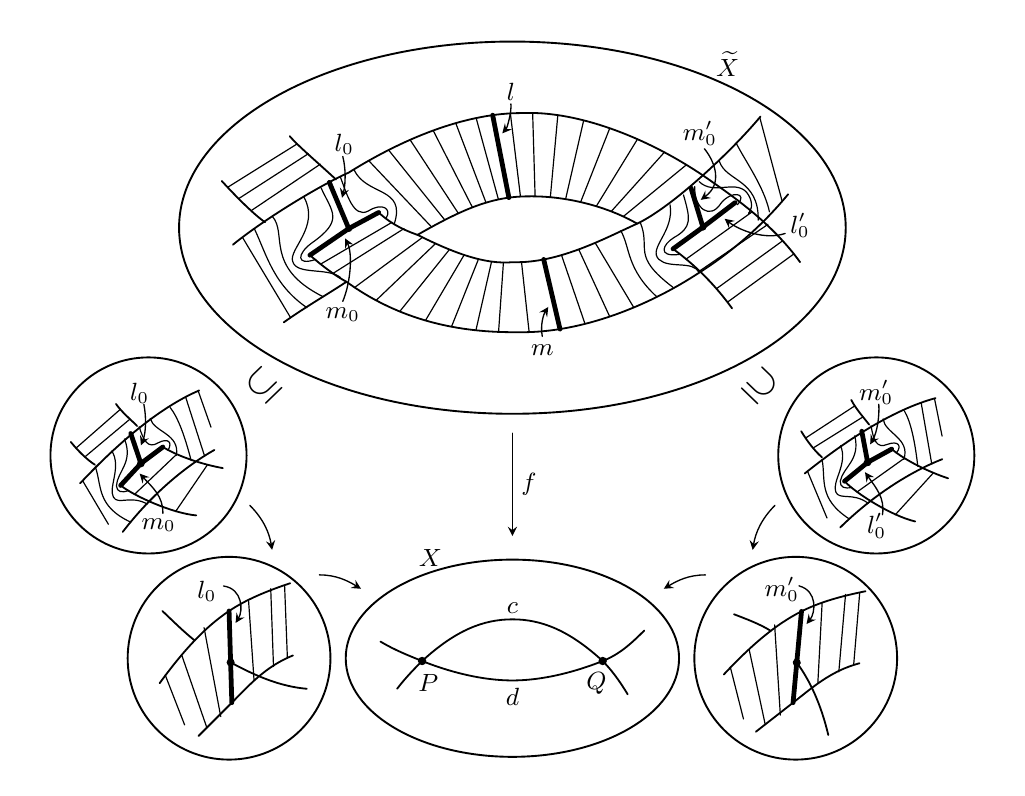
\begin{tikzpicture}[
    x=1bp, y=-1bp, line cap=round, line join=round, >=stealth,
    frame/.style={line width=.68bp},
    edge/.style={line width=.65bp},
    ruling/.style={line width=.43bp},
    fiber/.style={line width=1.72bp},
    leader/.style={->,line width=.48bp},
    every node/.style={font=\small,inner sep=0pt}
  ]
  \path[use as bounding box] (0,0) rectangle (349,266.4);

  \draw[frame] (174.5,72) ellipse[x radius=120, y radius=67];
  \draw[frame] (43.5,154) circle[radius=35.3];
  \draw[frame] (305.5,154) circle[radius=35.3];
  \draw[frame] (72.5,227) circle[radius=36.5];
  \draw[frame] (276.5,227) circle[radius=36.5];
  \draw[frame] (174.5,227) ellipse[x radius=60, y radius=35.5];

  % The two local views lie in the variety at the top.
  \node[rotate=44,font=\Large] at (85,129) {$\subseteq$};
  \node[rotate=-44,font=\Large] at (264,129) {$\supseteq$};
  \node at (252,13) {$\widetilde X$};

  % The ruled surface in the top view and its two local crossings.
  \begin{scope}[shift={(66.9,18.9)}, x=.269bp,y=-.252bp]
    \coordinate (back-left) at (181,132);
    \coordinate (back-right) at (667,145);
    \coordinate (front-left) at (178,288);
    \coordinate (front-right) at (650,275);
    \coordinate (inside-left) at (273,221);
    \coordinate (inside-right) at (567,205);
    \coordinate (left-junction) at (181,212);
    \coordinate (right-junction) at (655,210);

    % The four edges of the front and back bands.
    \draw[edge] (26,235)
      .. controls (70,197) and (143,150) .. (back-left)
      .. controls (262,78) and (343,47) .. (412,47)
      .. controls (495,43) and (595,90) .. (back-right);
    \draw[edge] (94,346)
      .. controls (123,324) and (151,307) .. (front-left)
      .. controls (250,344) and (330,361) .. (407,360)
      .. controls (492,362) and (583,322) .. (front-right)
      .. controls (691,247) and (732,211) .. (769,163);
    \draw[edge] (inside-left)
      .. controls (332,185) and (372,166) .. (421,166)
      .. controls (473,165) and (528,181) .. (inside-right);
    \draw[edge] (inside-left)
      .. controls (318,245) and (362,264) .. (401,260)
      .. controls (463,262) and (527,224) .. (inside-right)
      .. controls (614,181) and (693,102) .. (732,52);

    \draw[ruling]
      (207.7,115.0) -- (291.8,209.7)
      (234.3,99.8) -- (309.5,199.7)
      (263.1,85.2) -- (327.7,190.3)
      (294.0,71.9) -- (346.5,181.7)
      (324.2,61.4) -- (364.7,175.0)
      (351.5,54.1) -- (381.3,170.4)
      (397.3,47.5) -- (410.8,166.3)
      (427.1,46.8) -- (430.4,166.0)
      (460.8,49.9) -- (450.8,167.2)
      (495.4,57.4) -- (471.2,170.0)
      (530.3,68.7) -- (491.3,174.2)
      (567.4,84.3) -- (512.3,180.1)
      (603.4,103.0) -- (532.3,187.5)
      (632.9,120.9) -- (548.4,194.8)
      (188.9,296.1) -- (279.7,224.6)
      (217.6,314.6) -- (297.2,233.4)
      (249.2,330.5) -- (315.8,241.9)
      (283.7,343.3) -- (335.4,249.7)
      (318.5,352.2) -- (354.6,255.6)
      (351.2,357.3) -- (372.1,259.2)
      (381.5,359.6) -- (388.0,260.5)
      (422.4,359.9) -- (412.2,259.9)
      (497.2,348.2) -- (465.7,249.9)
      (530.2,337.7) -- (488.8,241.8)
      (562.4,324.7) -- (510.8,232.4);

    % Left patch. The diagonal strip is interrupted at the crossing.
    \draw[edge]
      (11,144) .. controls (29,165) and (53,191) .. (69,203)
      (102,80) .. controls (113,94) and (142,120) .. (164,142)
      (129,250) .. controls (145,265) and (165,281) .. (front-left)
      (221,189) .. controls (234,202) and (249,212) .. (inside-left);
    \draw[ruling]
      (19,153) -- (112,91)
      (34,169) -- (127,105)
      (51,186) -- (143,120)
      (143,263) -- (239,203)
      (160,276) -- (255,212)
      (39,225) -- (103,339)
      (55,213) .. controls (71,249) and (80,292) .. (125,325)
      (79,195) .. controls (99,219) and (68,267) .. (146,309)
      (121,167) .. controls (143,209) and (100,242) .. (106,259)
        .. controls (111,279) and (153,267) .. (170,282)
      (144,154) .. controls (159,189) and (175,200) .. (131,233)
        .. controls (112,248) and (110,266) .. (137,256)
      (170,139) .. controls (178,161) and (187,198) .. (207,187)
        .. controls (226,174) and (239,184) .. (231,197)
      (188,128) .. controls (205,166) and (258,152) .. (242,205);
    \draw[fiber]
      (155,146) -- (left-junction)
      (129,250) -- (left-junction) -- (221,189);
    \fill (left-junction) circle[radius=1.25bp];

    % Right patch, with the roles of the two fibers interchanged.
    \draw[edge]
      (back-right) .. controls (702,171) and (750,208) .. (785,260)
      (615,241) .. controls (647,266) and (673,295) .. (694,326);
    \draw[ruling]
      (632,256) -- (721,188)
      (650,273) -- (742,206)
      (673,298) -- (761,230)
      (688,317) -- (777,248)
      (731,53) -- (761,173)
      (700,91) .. controls (712,116) and (737,153) .. (744,188)
      (677,116) .. controls (686,145) and (730,141) .. (729,200)
      (650,145) .. controls (670,166) and (702,139) .. (716,164)
        .. controls (724,179) and (718,188) .. (716,190)
      (644,152) .. controls (643,184) and (665,200) .. (679,176)
        .. controls (693,157) and (716,161) .. (701,178)
      (629,164) .. controls (638,198) and (641,210) .. (616,225)
        .. controls (602,234) and (593,253) .. (623,249)
      (611,178) .. controls (617,217) and (581,240) .. (596,256)
        .. controls (610,270) and (642,257) .. (650,275)
      (571,203) .. controls (586,241) and (558,250) .. (615,296)
      (545,215) .. controls (558,239) and (552,269) .. (593.4,309.6);
    \draw[fiber]
      (639,154) -- (right-junction)
      (615,241) -- (right-junction) -- (698,175);
    \fill (right-junction) circle[radius=1.25bp];

    \draw[fiber]
      (373.6,50.0) -- (395.3,167.8)
      (463.7,355.6) -- (441.9,256.1);
    \node at (398,16) {$l$};
    \draw[leader] (398,34) .. controls (399,46) and (393,68) .. (386.5,76);
    \node at (440,385) {$m$};
    \draw[leader] (440,366) .. controls (437,349) and (442,334) .. (448,324);
    \node at (175,92) {$l_0$};
    \draw[leader] (173,109) .. controls (177,125) and (177,148) .. (172,168);
    \node at (173,335) {$m_0$};
    \draw[leader] (173,316) .. controls (184,288) and (186,247) .. (176,226);
    \node at (651,76) {$m'_0$};
    \draw[leader] (657,98) .. controls (672,118) and (681,148) .. (652,171);
    \node at (785,208) {$l'_0$};
    \draw[leader] (765,219) .. controls (738,229) and (703,214) .. (684,198);
  \end{scope}

  % The two intermediate views share the local geometry, with exchanged labels.
  \def\DrawDoublePatch#1#2{%
    \begin{scope}[x=.152bp,y=-.152bp]
      \begin{scope}[shift={(-218,-218)}]
        \coordinate (junction) at (200,237);
        \draw[edge]
          (56,284) .. controls (112,225) and (222,114) .. (338,64)
          (157,399) .. controls (223,313) and (303,245) .. (374,205)
          (34,186) .. controls (49,205) and (72,228) .. (91,240)
          (141,96) .. controls (154,115) and (179,136) .. (191,148)
          (152,289) .. controls (185,315) and (275,355) .. (331,360)
          (252,198) .. controls (291,222) and (350,240) .. (394,248);
        \draw[ruling]
          (47,200) -- (151,109)
          (69,220) -- (174,132)
          (185,310) -- (284,216)
          (282,351) -- (357,241)
          (62,278) -- (123,381)
          (92,245) .. controls (108,290) and (94,338) .. (176,376)
          (131,207) .. controls (155,246) and (122,294) .. (135,317)
            .. controls (146,336) and (175,311) .. (215,333)
          (161,179) .. controls (183,234) and (144,256) .. (142,290)
            .. controls (143,305) and (155,307) .. (171,301)
          (196,150) .. controls (206,183) and (217,203) .. (241,188)
            .. controls (264,176) and (276,186) .. (264,206)
          (222,130) .. controls (230,163) and (293,166) .. (284,218)
          (269,104) .. controls (288,128) and (304,172) .. (319,230)
          (306,80) -- (351,220)
          (336,66) -- (366,151);
        \draw[fiber]
          (176,166) -- (junction)
          (152,289) -- (junction) -- (252,198);
        \fill (junction) circle[radius=1.4bp];
        \node at (197,71) {$#1$};
        \draw[leader] (207,97) .. controls (213,126) and (212,164) .. (200,194);
        \node at (242,383) {$#2$};
        \draw[leader] (252,355) .. controls (253,315) and (227,293) .. (197,261);
      \end{scope}
    \end{scope}%
  }
  \begin{scope}[shift={(43.5,154)}]
    \DrawDoublePatch{l_0}{m_0}
  \end{scope}
  \begin{scope}[shift={(305.5,154)},rotate=-8]
    \DrawDoublePatch{m'_0}{l'_0}
  \end{scope}

  % The first blow-up in each neighborhood, before the second curve is blown up.
  \def\DrawFirstPatch#1#2{%
    \coordinate (on-fiber) at (.56,1.5);
    \draw[edge]
      (-25,9) .. controls (-17,-2) and (-9,-11) .. (0,-17)
        coordinate[pos=.52] (left-entry) coordinate[pos=.61] (right-entry)
        .. controls (6,-21) and (13,-24) .. (22,-27)
      (-11,28) .. controls (-7,24) and (-3,20) .. (1,16)
        .. controls (7,10) and (13,3) .. (23,-1);
    % Only the parts of the transverse curve visible past the band are drawn.
    \draw[edge] #2;
    \draw[ruling]
      (-23,6) -- (-16,24)
      (-17,-1) -- (-8,25)
      (-9,-11) -- (-3,21)
      (7,-21) -- (9,8)
      (15,-25) -- (16,3)
      (20,-26) -- (21,0);
    \draw[fiber] (0,-17) -- (1,16);
    \fill (on-fiber) circle[radius=1.45bp];
    \node at (-8,-24) {$#1$};
    \draw[leader] (-2,-26) .. controls (5,-25) and (5,-17) .. (2.35,-12.7);
  }
  \begin{scope}[shift={(72.5,227)}]
    \DrawFirstPatch{l_0}{
      (-24,-17) .. controls (-20.1,-13.3) and (-16.4,-9.6) .. (left-entry)
      (on-fiber) .. controls (9.6,6.4) and (18.5,10.2) .. (28,11)
    }
  \end{scope}
  \begin{scope}[shift={(276.5,227)},rotate=-7]
    \DrawFirstPatch{m'_0}{
      (-24,-13) .. controls (-20,-12) and (-14,-10.6) .. (right-entry)
      (on-fiber) .. controls (6,7.3) and (11,15.2) .. (15,26)
    }
  \end{scope}

  % The four local maps and the global map f.
  \draw[leader] (80,172) .. controls (85,177) and (87,182) .. (88,188);
  \draw[leader] (269,172) .. controls (264,177) and (262,182) .. (261,188);
  \draw[leader] (105,197) .. controls (111,197) and (115,199) .. (120,202);
  \draw[leader] (244,197) .. controls (238,197) and (234,199) .. (229,202);
  \draw[leader] (174.5,146) -- node[right=3bp] {$f$} (174.5,183);

  % The two curves c and d in X.
  \coordinate (P) at (142,228);
  \coordinate (Q) at (207,228);
  \draw[edge] (133,238)
    .. controls (136,234) and (140,230) .. (P)
    .. controls (154,217) and (164,213) .. (174.5,213)
    .. controls (185,213) and (195,217) .. (Q)
    .. controls (210,231) and (213,235) .. (216,240);
  \draw[edge] (127,221)
    .. controls (132,224) and (137,226) .. (P)
    .. controls (151,231.6) and (163,235) .. (174.5,235)
    .. controls (186,235) and (198,231.6) .. (Q)
    .. controls (213,225.6) and (217,222) .. (222,217);
  \fill (P) circle[radius=1.52bp];
  \fill (Q) circle[radius=1.52bp];
  \node at (145,191) {$X$};
  \node at (174.5,209) {$c$};
  \node at (174.5,241) {$d$};
  \node at (144.2,236) {$P$};
  \node at (204.8,236) {$Q$};
\end{tikzpicture}
}\par
\noindent\hypertarget{fig-book-24}{}\small Figure 24.\quad A complete nonprojective variety.\par}
}
% Contents from body/page-458.tex.
\ChapterSheet{458}{444}{\Goto{p-452}{Appendix B\quad Transcendental Methods}}{%
blow up the curve $d$, then blow up the strict transform of the curve $c$. On $X-P-Q$ it doesn't matter in which order we blow up the curves $c$ and $d$, so we can glue our blown-up varieties along the inverse images of $X-P-Q$. The result is a nonsingular complete algebraic variety $\widetilde X$. We will show that $\widetilde X$ is not projective. It follows, incidentally, that the birational morphism $f\colon\widetilde X\to X$ cannot be factored into any sequence of monoidal transformations, because it is not a projective morphism.

To do this, we must examine what happens in a neighborhood of $P$ (Fig.~\Goto{fig-book-24}{24}). Let $l$ be the inverse image in $\widetilde X$ of a general point of $c$. Let $m$ be the inverse image of a general point of $d$. Note that $l$ and $m$ are projective lines. Then the inverse image of $P$ consists of two lines $l_0$ and $m_0$, and we have algebraic equivalence of cycles $l\sim l_0+m_0$ and $m\sim m_0$. Note the asymmetry resulting from the order in which we blew up the two curves. Now in the neighborhood of $Q$ the opposite happens. So $f^{-1}(Q)$ is the union of two lines $l'_0$ and $m'_0$, and we have algebraic equivalence $l\sim \EditionText{l'_0}$ and $m\sim l'_0+m'_0$. Combining these equivalences, we find that $l_0+m'_0\sim0$. This would be impossible on a projective variety, because a curve has a degree, which is a positive integer, and degrees are additive and are preserved by algebraic equivalence. So $\widetilde X$ is not projective.

\medskip
\noindent\hypertarget{result-B-3.4.2}{}\textbf{Example 3.4.2.} For the second example, we start with any nonsingular projective algebraic threefold, as before. Let $c$ be \EditionText{an integral curve} in $X$ which is nonsingular except for one double point $P$, having distinct tangent directions. In a small analytic neighborhood of $P$, blow up one branch first, then the other. Outside of that neighborhood, just blow up $c$. Then glue to obtain the compact complex manifold $\mathfrak X$. Clearly $\mathfrak X$ is Moishezon, because the meromorphic functions on $\mathfrak X$ are the same as those on $X$. We will show that $\mathfrak X$ is not an abstract algebraic variety.

Using the same notation as before (Fig.~\Goto{fig-book-25}{25}) we have homological equivalences $l\sim l_0+m_0$, $m\sim m_0$, and $l\sim m$, because \EditionText{the two general fibre lines lie in the same $\Proj^1$-bundle}

\smallskip
{\centering
\noindent\resizebox{\linewidth}{!}{% Figure 25. A nonalgebraic Moishezon manifold (printed page 444).
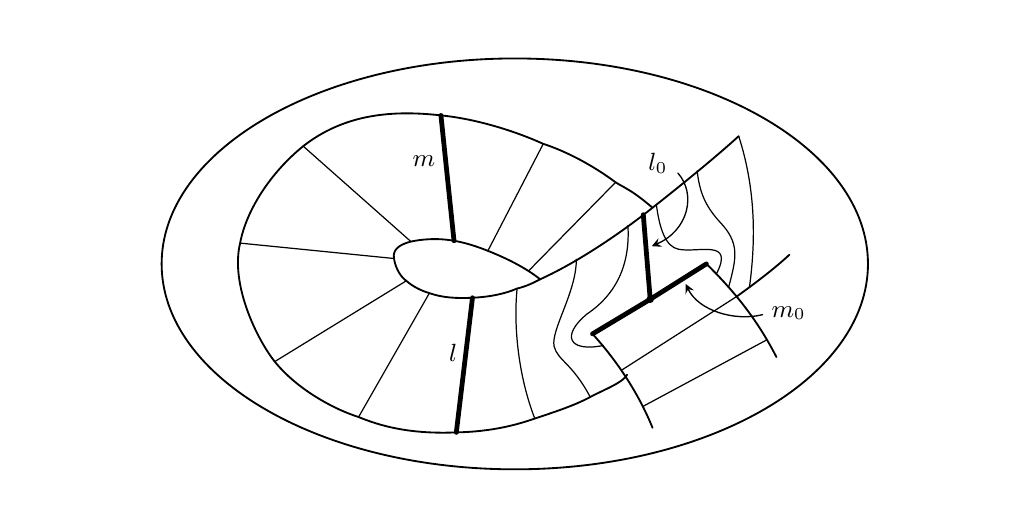
\begin{tikzpicture}[
    x=.277bp, y=-.277bp, line cap=round, line join=round, >=stealth,
    edge/.style={line width=.66bp},
    ruling/.style={line width=.44bp},
    fiber/.style={line width=1.72bp},
    leader/.style={->,line width=.48bp},
    every node/.style={font=\small,inner sep=0pt}
  ]
  \path[use as bounding box] (-162.1,-28) rectangle (1097.828,556.116);
  \draw[edge] (471,279) ellipse[x radius=459,y radius=267];

  \coordinate (join) at (504,299);
  \coordinate (upper-m) at (375,86);
  \coordinate (lower-m) at (392,249);
  \coordinate (upper-l) at (416,323);
  \coordinate (lower-l) at (395,498);
  \coordinate (double-point) at (647,325);
  \coordinate (rim-start) at (650,206);

  % The outer rim of the ruled band and the edge of the central opening.
  \draw[edge] (rim-start)
    .. controls (623,183) and (615,181) .. (602,173)
    .. controls (574,152) and (539,133) .. (508,123)
    .. controls (466,104) and (416,90) .. (upper-m)
    .. controls (305,78) and (246,87) .. (196,126)
    .. controls (154,160) and (122,209) .. (114,252)
    .. controls (101,306) and (136,377) .. (159,406)
    .. controls (188,442) and (236,468) .. (268,478)
    .. controls (306,494) and (347,500) .. (lower-l)
    .. controls (442,497) and (474,488) .. (497,480)
    .. controls (521,472) and (549,463) .. (569,452)
    .. controls (588,442) and (612,433) .. (617,423);
  \draw[edge] (join)
    .. controls (485,284) and (461,272) .. (436,262)
    .. controls (421,256) and (405,251) .. (lower-m)
    .. controls (370,245) and (350,247) .. (336,250)
    .. controls (320,254) and (312,261) .. (314,272)
    .. controls (316,286) and (324,297) .. (330,301)
    .. controls (339,309) and (350,314) .. (360,317)
    .. controls (377,323) and (395,324) .. (upper-l)
    .. controls (438,322) and (458,318) .. (474,311)
    .. controls (487,308) and (496,303) .. (join)
    .. controls (561,273) and (620,230) .. (rim-start)
    .. controls (683,180) and (729,143) .. (762,113);

  \draw[ruling]
    (196,126) -- (336,250)
    (114,252) -- (314,272)
    (159,406) -- (330,301)
    (268,478) -- (360,317)
    (508,123) -- (436,262)
    (602,173) -- (489,288)
    (474,311) .. controls (469,361) and (476,426) .. (497,480);

  % The two strips meeting in the exceptional fibers.
  \draw[edge]
    (572,370) .. controls (602,403) and (631,445) .. (650,492)
    (720,279) .. controls (759,317) and (788,355) .. (811,400)
    (760,321) .. controls (785,303) and (811,283) .. (828,267);
  \draw[ruling]
    (610,417) -- (760,321)
    (638,464) -- (798,378)
    (551,273) .. controls (551,316) and (518,364) .. (522,386)
      .. controls (527,405) and (545,407) .. (569,452)
    (618,229) .. controls (621,277) and (605,317) .. (565,344)
      .. controls (530,373) and (542,394) .. (586,385)
    (655,202) .. controls (659,233) and (667,257) .. (684,260)
      .. controls (709,265) and (757,246) .. (733,292)
    (708,158) .. controls (711,185) and (718,203) .. (737,224)
      .. controls (764,252) and (759,271) .. (749,309)
    (762,113) .. controls (783,178) and (785,243) .. (776,309);

  \draw[fiber]
    (upper-m) -- (lower-m)
    (upper-l) -- (lower-l)
    (638,215) -- (double-point)
    (572,370) -- (double-point) -- (720,279);
  \fill (double-point) circle[radius=1.35bp];

  \node at (353,145) {$m$};
  \node at (391,394) {$l$};
  \node at (657,148) {$l_0$};
  \node[anchor=west] at (804,343) {$m_0$};
  \draw[leader] (683,161)
    .. controls (707,188) and (697,235) .. (649,256);
  \draw[leader] (793,345)
    .. controls (757,354) and (710,340) .. (693,305);
\end{tikzpicture}
}\par
\noindent\hypertarget{fig-book-25}{}\small Figure 25.\quad A nonalgebraic Moishezon manifold.\par}
}
% Contents from body/page-459.tex.
\BookMark{1}{B.4  K\"ahler Manifolds}{sec-B-4}
\ChapterSheet{459}{445}{\Goto{sec-B-4}{4\quad K\"ahler Manifolds}}{%
\EditionText{over the connected smooth locus $c-\{P\}$.} So we find that $l_0\sim0$. But this is impossible if $\mathfrak X$ is algebraic. Indeed, let $T$ be a point of $l_0$. Then $T$ has an affine neighborhood $U$ in $\mathfrak X$. Let $Y$ be an irreducible surface in $U$ which passes through $T$ but does not contain $l_0$. Extend $Y$ by closure to a surface $Y$ in $\mathfrak X$. Now $Y$ meets $l_0$ in a finite nonzero number of points, so the intersection number of $Y$ with $l_0$ is defined and is $\ne0$. But the intersection number is defined on homology classes, so we cannot have $l_0\sim0$. Hence $\mathfrak X$ is not algebraic.

\medskip
\noindent\hypertarget{result-B-3.4.3}{}\textbf{Remark 3.4.3.} At this point we should also mention the algebraic spaces of Artin \Goto{bib-artin-2}{[2]} and Knutson \Goto{bib-knutson-1}{[1]}. Over any field $k$, they define an \emph{algebraic space} to be something which is locally a quotient of a scheme by an \'etale equivalence relation. The category of algebraic spaces contains the category of schemes. If $X$ is an algebraic space of finite type over $\mathbb C$, one can define its associated complex analytic space $X_h$. Artin shows that the category of smooth proper algebraic spaces over $\mathbb C$ is equivalent, via the functor $h$, to the category of Moishezon manifolds. Thus every Moishezon manifold is \textquotedblleft{}algebraic\textquotedblright{}\ in the sense of algebraic spaces. In particular, Hironaka's example \Goto{result-B-3.4.2}{(3.4.2)} gives an example of an algebraic space over $\mathbb C$ which is not a scheme.

\bigskip
\noindent\hypertarget{sec-B-4}{}{\large\bfseries 4\quad K\"ahler Manifolds}\par
\medskip
\noindent The methods of differential geometry provide a powerful tool for the study of compact complex manifolds, and hence of algebraic varieties over the complex numbers. Notable among such applications of differential geometry are Hodge's \Goto{bib-hodge-1}{[1]} theory of harmonic integrals, and the resulting decomposition of the complex cohomology into its $(p,q)$-components (see also Weil \Goto{bib-483-8}{[5]}); the vanishing theorems of Kodaira \Goto{bib-kodaira-1}{[1]} and Nakano \Goto{bib-nakano-1}{[1]}, recently generalized by Grauert and Riemenschneider \Goto{bib-grauert-riemenschneider-1}{[1]}; and the work of Griffiths on the intermediate Jacobians and the period mapping. Here we will only mention the definition of a K\"ahler manifold, and how that notion helps to characterize algebraic complex manifolds.

Any complex manifold admits a Hermitian metric (in many ways). A Hermitian metric is said to be \emph{K\"ahler} if the associated differential $2$-form of type $(1,1)$ is closed. A complex manifold with a K\"ahler metric is called a \emph{K\"ahler manifold}. One can show easily that complex projective space has a natural K\"ahler metric on it, and hence that every projective algebraic manifold is a K\"ahler manifold with the induced metric. \EditionText{A compact complex manifold $\mathfrak X$ is called a \emph{Hodge manifold} if it admits a K\"ahler metric whose associated $2$-form has cohomology class in the image of $H^2(\mathfrak X,\mathbb Z)\to H^2(\mathfrak X,\mathbb C)$.} Now a fundamental result is

\medskip
\noindent\hypertarget{result-B-4.1}{}\textbf{Theorem 4.1} (Kodaira \Goto{bib-478-16}{[2]}). \emph{Every Hodge manifold is projective algebraic.}
}
% Contents from body/page-460.tex.
\BookMark{1}{B.5  The Exponential Sequence}{sec-B-5}
\ChapterSheet{460}{446}{\Goto{p-452}{Appendix B\quad Transcendental Methods}}{%
\indent This can be thought of as a generalization of the theorem of Riemann \Goto{result-B-3.1}{(3.1)} quoted above, because \EditionText{a Hermitian $2$-form on a compact connected complex manifold of dimension one is closed and can be scaled to have total area one, hence integral cohomology class.} We also have the following

\medskip
\noindent\hypertarget{result-B-4.2}{}\textbf{Theorem 4.2} (Moishezon \Goto{bib-480-0}{[2]}). \emph{Every Moishezon manifold which is K\"ahler is projective algebraic.}

\medskip
Summing up, we have the following implications among properties of compact complex manifolds, and there are examples to show that no further implications are possible.
\begin{center}
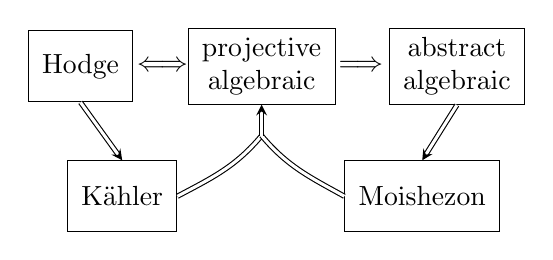
\begin{tikzpicture}[x=1cm,y=1cm,
    property/.style={draw,align=center,minimum height=.9cm,inner xsep=5pt},
    implication/.style={double,double distance=1.1pt,-stealth}]
  \node[property] (H) at (-2.5,0) {Hodge};
  \node[property] (P) at (-.2,0) {projective\\algebraic};
  \node[property] (A) at (2.28,0) {abstract\\algebraic};
  \node[property] (K) at (-1.97,-1.65) {K\"ahler};
  \node[property] (M) at (1.84,-1.65) {Moishezon};
  \node at (-1.46,0) {$\Longleftrightarrow$};
  \node at (1.06,0) {$\Longrightarrow$};
  \draw[implication] (H.south) -- (K.north);
  \draw[implication] (A.south) -- (M.north);
  \draw[double,double distance=1.1pt] (K.east) to[out=28,in=230] (-.2,-.88);
  \draw[double,double distance=1.1pt] (M.west) to[out=151,in=310] (-.2,-.88);
  \draw[implication] (-.2,-.89) -- (P.south);
\end{tikzpicture}
\end{center}

\medskip
\noindent\hypertarget{sec-B-5}{}{\large\bfseries 5\quad The Exponential Sequence}\par
\medskip
\noindent Let us give one simple example of the use of transcendental methods, by looking at the exponential sequence. The exponential function $f(x)=e^{2\pi ix}$ gives an exact sequence of abelian groups
\[
0\to\mathbb Z\to\mathbb C\xrightarrow{f}\mathbb C^*\to0,
\]
where $\mathbb C$ has its additive structure, and $\mathbb C^*=\mathbb C-\{0\}$ has its multiplicative structure. If $\mathfrak X$ is any reduced complex analytic space, by considering holomorphic functions with values in the above sequence, we get an exact sequence of sheaves
\[
0\to\mathbb Z\to\mathcal O_{\mathfrak X}\xrightarrow{f}\mathcal O_{\mathfrak X}^*\to0,
\]
where $\mathbb Z$ is the constant sheaf, $\mathcal O_{\mathfrak X}$ is the structure sheaf, and $\mathcal O_{\mathfrak X}^*$ is the sheaf of invertible elements of $\mathcal O_{\mathfrak X}$ under multiplication.

The cohomology sequence of this short exact sequence of sheaves is very interesting. Let us apply it to $X_h$, where $X$ is a projective variety over $\mathbb C$. At the $H^0$ level, we recover the original exact sequence of groups $0\to\mathbb Z\to\mathbb C\to\mathbb C^*\to0$, because the global holomorphic functions are constant. Then starting with $H^1$, we have an exact sequence
\[
\begin{gathered}
0\to H^1(X_h,\mathbb Z)\to H^1(X_h,\mathcal O_{X_h})\to H^1(X_h,\mathcal O_{X_h}^*)\\
\to H^2(X_h,\mathbb Z)\to H^2(X_h,\mathcal O_{X_h})\to\cdots\,.
\end{gathered}
\]
By Serre's theorem \Goto{result-B-2.1}{(2.1)}, we have $H^i(X_h,\mathcal O_{X_h})\cong H^i(X,\mathcal O_X)$. On the other hand
\[
H^1(X_h,\mathcal O_{X_h}^*)\cong\operatorname{Pic}X_h
\]
}
% Contents from body/page-461.tex.
\ChapterSheet[\EditionText{10.9}]{461}{447}{\Goto{sec-B-5}{5\quad The Exponential Sequence}}{%
by (III, Ex.~\Goto{ex-III-4.5}{4.5}), which is valid for any ringed space. But Serre's theorem \Goto{result-B-2.1}{(2.1)} also gives an equivalence of categories of coherent sheaves, so in particular, $\operatorname{Pic} X_h\cong\operatorname{Pic} X$. So we can rewrite our sequence as
\[
0\to H^1(X_h,\mathbb Z)\to H^1(X,\mathcal O_X)\to\operatorname{Pic} X\to H^2(X_h,\mathbb Z)\to H^2(X,\mathcal O_X)\to\cdots\,.
\]

The only nonalgebraic part is the integral cohomology of $X_h$. Since any algebraic variety is triangulable (see for example, Hironaka \Goto{bib-hironaka-5}{[5]}), the cohomology groups $H^i(X_h,\mathbb Z)$ are finitely generated abelian groups. From this sequence we can deduce some information about the Picard group of $X$.

First of all, one sees easily that algebraically equivalent Cartier divisors give the same element in $H^2(X_h,\mathbb Z)$. \EditionText{The kernel of $c_1\colon\operatorname{Pic}X\to H^2(X_h,\mathbb Z)$ is the image of $H^1(X,\mathcal O_X)$ by exactness, and this image equals $\operatorname{Pic}^{\circ}X$, the group of divisors algebraically equivalent to zero modulo linear equivalence. Thus the N\'eron--Severi group of $X$ is a subgroup of $H^2(X_h,\mathbb Z)$, and hence is finitely generated (V, Ex.~\Goto{ex-V-1.7}{1.7}). When $X$ is nonsingular, the quotient $\operatorname{Pic}^{\circ}X\cong H^1(X,\mathcal O_X)/H^1(X_h,\mathbb Z)$ is a complex torus and in fact an abelian variety, the \emph{Picard variety} of $X$.}

If $X$ is a nonsingular curve of genus $g$, we can see even more clearly what is happening. In that case $X_h$ is a compact Riemann surface of genus $g$. As a topological space, it is a compact oriented real $2$-manifold which is homeomorphic to a sphere with $g$ handles. So we have
\[
H^0(X_h,\mathbb Z)=H^2(X_h,\mathbb Z)=\mathbb Z,
\qquad\text{and}\qquad
H^1(X_h,\mathbb Z)\cong\mathbb Z^{2g}.
\]
On the other hand, $H^1(X,\mathcal O_X)\cong\mathbb C^g$, so
\[
\operatorname{Pic}^{\circ} X\cong\mathbb C^g/\mathbb Z^{2g}.
\]
This is the Jacobian variety of $X$ (IV, \Goto{sec-IV-4}{\S4}), which is an abelian variety of dimension $g$. Of course $\operatorname{NS}(X)\cong\mathbb Z$ in this case, the isomorphism being given by the degree function.

\medskip
\noindent\hypertarget{sec-B-6}{}\textsc{Exercises}\par
\smallskip
{\fontsize{9.15}{10.4}\selectfont\setlength{\parskip}{.9pt}\leftskip=21pt
\noindent\hypertarget{ex-B-6.1}{}\llap{\textbf{6.1.}\enspace}Show that the unit disc in $\mathbb C$ is not isomorphic to $X_h$ for any scheme $X$.

\smallskip
\noindent\hypertarget{ex-B-6.2}{}\llap{\textbf{6.2.}\enspace}Let $z_1,z_2,\ldots$ be an infinite sequence of complex numbers with $|z_n|\to\infty$ as $n\to\infty$. Let $\mathfrak I\subseteq\mathcal O_{\mathbb C}$ be the sheaf of ideals of holomorphic functions vanishing at all of the $z_n$. Show that there is no coherent algebraic sheaf of ideals $\mathcal I\subseteq\mathcal O_X$, where $X=\AffSpace{1}_{\mathbb C}$ is the affine line, such that $\mathfrak I=\mathcal I_h$ as an ideal in $\mathcal O_{\mathbb C}$. Show on the other hand that there is a coherent sheaf $\mathcal F$ on $X$ such that $\mathcal F_h\cong\mathfrak I$ as coherent sheaves.

\smallskip
\noindent\hypertarget{ex-B-6.3}{}\llap{\textbf{6.3.}\enspace}(Serre \Goto{bib-482-0}{[12]}.) On $\mathbb C^2-\{0,0\}$, we define an invertible analytic sheaf $\mathfrak L$ as follows: $\mathfrak L\cong\mathcal O$ when $z\ne0$; $\mathfrak L\cong\mathcal O$ when $w\ne0$, and when both $z,w\ne0$, the two copies of $\mathcal O$ are glued by multiplication by $e^{-1/(zw)}$ in the local ring at the point $(z,w)$. Show that there is no invertible algebraic sheaf $\mathcal L$ on $\AffSpace{2}-\{0,0\}$ with $\mathcal L_h\cong\mathfrak L$.

\smallskip
\noindent\hypertarget{ex-B-6.4}{}\llap{\textbf{6.4.}\enspace}Show directly that if $X$ is a scheme which is reduced and proper over $\mathbb C$, then $H^0(X,\mathcal O_X)\cong H^0(X_h,\mathcal O_{X_h})$. \EditionText{Conversely, show that if $X$ is separated and of finite type over $\mathbb C$ but is not proper, there is a coherent sheaf $\mathcal F$ for which $H^0(X,\mathcal F)\to H^0(X_h,\mathcal F_h)$ is not surjective.}\par}
}
% Contents from body/page-462.tex.
\ChapterSheet{462}{448}{\Goto{p-452}{Appendix B\quad Transcendental Methods}}{%
{\fontsize{9.15}{10.4}\selectfont\setlength{\parskip}{.9pt}\leftskip=21pt
\noindent\hypertarget{ex-B-6.5}{}\llap{\textbf{6.5.}\enspace}If $X,X'$ are nonsingular affine algebraic curves, with $X_h\cong X_h'$, show that $X\cong X'$.

\smallskip
\noindent\hypertarget{ex-B-6.6}{}\llap{\textbf{6.6.}\enspace}Show that if $X$ and $Y$ are projective schemes over $\mathbb C$, and $\mathfrak f\colon X_h\to Y_h$ is a morphism of analytic spaces, then there exists a (unique) morphism $f\colon X\to Y$ with $f_h=\mathfrak f$. [\emph{Hint:} First reduce to the case $Y=\Proj^n$. Then consider the invertible analytic sheaf $\mathfrak L=\mathfrak f^*\mathcal O(1)$ on $X_h$, use \Goto{result-B-2.1}{(2.1)}, and the techniques of (II, \Goto{sec-II-7}{\S7}).]\par}
}
% Contents from body/page-463.tex.
% Original printed page 449.
\BookMark{0}{Appendix C  The Weil Conjectures}{p-463}
\BookMark{1}{C.1  The Zeta Function and the Weil Conjectures}{sec-C-1}
\ChapterSheet[11.10]{463}{449}{}{%
\vspace*{22pt}%
\noindent{\large\bfseries Appendix C}\par\vspace{3pt}%
\hrule
\vspace{6pt}%
\noindent{\Large\bfseries The Weil Conjectures}\par
\vspace{146pt}%

\noindent In 1949, Andr\'e Weil \Goto{bib-483-7}{[4]} stated his now famous conjectures concerning the number of solutions of polynomial equations over finite fields. These conjectures suggested a deep connection between the arithmetic of algebraic varieties defined over finite fields and the topology of algebraic varieties defined over the complex numbers. Weil also pointed out that if one had a suitable cohomology theory for abstract varieties, analogous to the ordinary cohomology of varieties defined over $\mathbf C$, then one could deduce his conjectures from various standard properties of the cohomology theory. This observation has been one of the principal motivations for the introduction of various cohomology theories into abstract algebraic geometry. In 1963, Grothendieck was able to show that his $\ell$-adic cohomology had sufficient properties to imply part of the Weil conjectures (the rationality of the zeta function). Deligne's \Goto{bib-475-4}{[3]} proof in 1973 of the remainder of the Weil conjectures (specifically the analogue of the \textquotedblleft Riemann hypothesis\textquotedblright) may be regarded as the culmination of the study of $\ell$-adic cohomology begun by Grothendieck, M. Artin, and others in the Paris seminars \Goto{bib-SGA-4}{[SGA 4]}, \Goto{bib-SGA-5}{[SGA 5]}, and \Goto{bib-SGA-7}{[SGA 7]}.

\par\medskip
\noindent\AuditItem{sec-C-1}{1\quad The Zeta Function and the Weil Conjectures}\par\medskip
\noindent Let $k=\mathbf F_q$ be a finite field with $q$ elements. Let $X$ be a scheme of finite type over $k$. For example, $X$ could be the set of solutions in affine or projective space over $k$ of a finite number of polynomial equations with coefficients in $k$. Let $\overline k$ be an algebraic closure of $k$, and let $\overline X=X\times_k\overline k$ be the corresponding scheme over $\overline k$. \EditionText{For each integer $r\geq 1$, let $N_r=\#X(k_r)$, where $k_r=\mathbf F_{q^r}\subseteq\overline k$ and $X(k_r)=\operatorname{Hom}_k(\operatorname{Spec}k_r,X)$. Under the identification $X(\overline k)=\overline X(\overline k)$, these are precisely the points fixed by the $r$th power of the $q$-power Frobenius associated with $X$.}
}
% Contents from body/page-464.tex.
% Original printed page 450.
\ChapterSheet[11.10]{464}{450}{\Goto{p-463}{Appendix C\quad The Weil Conjectures}}{%
\noindent The numbers $N_1,N_2,N_3,\ldots$ are clearly of great importance in studying arithmetical properties of the scheme $X$. To study them, we form the \emph{zeta function} of $X$ (following Weil), which is defined as
\[
 Z(t)=Z(X;t)=\exp\!\left(\sum_{r=1}^{\infty}N_r\frac{t^r}{r}\right).
\]
Note that by definition, it is a power series with rational coefficients: $Z(t)\in\mathbf Q[[t]]$.

For example, let $X=\mathbf P^1$. Over any field, $\mathbf P^1$ has one more point than the number of elements of the field. Hence $N_r=q^r+1$. Thus
\[
 Z(\mathbf P^1,t)=\exp\!\left(\sum_{r=1}^{\infty}(q^r+1)\frac{t^r}{r}\right).
\]
It is easy to sum this series, and we find that
\[
 Z(\mathbf P^1,t)=\frac{1}{(1-t)(1-qt)}.
\]
In particular, it is a rational function of $t$.

\medskip
Now we can state the Weil conjectures. Let $X$ be a smooth \EditionText{geometrically connected }projective variety of dimension $n$ defined over $k=\mathbf F_q$. Let $Z(t)$ be the zeta function of $X$. Then

\medskip
\AuditItem{ex-C-1.1}{1.1.} \emph{Rationality.} $Z(t)$ is a rational function of $t$, i.e., a quotient of polynomials with rational coefficients.

\medskip
\AuditItem{ex-C-1.2}{1.2.} \emph{Functional equation.} Let $E$ be the self-intersection number of the diagonal $\Delta$ of $X\times X$ (which is also the \EditionText{degree of the top Chern class} of the tangent bundle of $X$ (App.~A, Ex.~\Goto{ex-A-6.6}{6.6})). Then $Z(t)$ satisfies a functional equation, namely
\[
 Z\!\left(\frac{1}{q^nt}\right)=\pm q^{nE/2}t^E Z(t).
\]

\medskip
\AuditItem{ex-C-1.3}{1.3.} \emph{Analogue of the Riemann hypothesis.} It is possible to write
\[
 Z(t)=\frac{P_1(t)P_3(t)\cdots P_{2n-1}(t)}
 {P_0(t)P_2(t)\cdots P_{2n}(t)}
\]
where $P_0(t)=1-t$; $P_{2n}(t)=1-q^nt$; and for each $1\leq i\leq 2n-1$, $P_i(t)$ is a polynomial with integer coefficients, which can be written
\[
 P_i(t)=\prod_j(1-\alpha_{ij}t),
\]
where the $\alpha_{ij}$ are algebraic integers with $|\alpha_{ij}|=q^{i/2}$. (Note that these conditions uniquely determine the polynomials $P_i(t)$, if they exist.)
}
% Contents from body/page-465.tex.
% Original printed page 451.
\BookMark{1}{C.2  History of Work on the Weil Conjectures}{sec-C-2}
\ChapterSheet[11.10]{465}{451}{\Goto{sec-C-2}{2\quad History of Work on the Weil Conjectures}}{%
\AuditItem{ex-C-1.4}{1.4.} \emph{Betti numbers.} Assuming \Goto{ex-C-1.3}{(1.3)}, we can define the $i$th Betti number $B_i=B_i(X)$ to be the degree of the polynomial $P_i(t)$. Then we have $E=\sum(-1)^iB_i$. Furthermore, suppose that $X$ is obtained from a variety $Y$ defined over an algebraic number ring $R$, by reduction modulo a prime ideal $\mathfrak p$ of $R$\EditionText{, and that $Y$ gives a smooth proper model over $R_{\mathfrak p}$}. Then $B_i(X)$ is equal to the $i$th Betti number of the topological space $Y_h=(Y\times_R\mathbf C)_h$ (App.~\Goto{p-452}{B}), i.e., $B_i(X)$ is the rank of the ordinary cohomology group $H^i(Y_h,\mathbf Z)$.

\medskip
Let us verify the conjectures for the case $X=\mathbf P^1$. We have already seen that $Z(t)$ is rational. The invariant $E$ of $\mathbf P^1$ is $2$, and one verifies immediately the functional equation which says in this case
\[
 Z\!\left(\frac{1}{qt}\right)=qt^2Z(t).
\]
The analogue of the Riemann hypothesis is immediate, with $P_1(t)=1$. Hence $B_0=B_2=1$ and $B_1=0$. These are indeed the usual Betti numbers of $\mathbf P_{\mathbf C}^1$, which is a sphere, and finally we have $E=\sum(-1)^iB_i$.

\par\bigskip
\AuditItem{sec-C-2}{2\quad History of Work on the Weil Conjectures}\par\medskip
\noindent Weil was led to his conjectures by consideration of the zeta functions of some special varieties. See his article Weil \Goto{bib-483-7}{[4]} for number-theoretic background, and calculations for the \textquotedblleft Fermat hypersurfaces\textquotedblright\ $\sum a_ix_i^n=0$. One of Weil's major pieces of work was the proof that his conjectures hold for curves. This is done in his book Weil \Goto{bib-weil-2}{[2]}. The rationality and the functional equation follow from the Riemann--Roch theorem on the curve. The analogue of the Riemann hypothesis is deeper (V, Ex.~\Goto{ex-V-1.10}{1.10}). He deduces it from an inequality of Castelnuovo and Severi about correspondences on a curve (V, Ex.~\Goto{ex-V-1.9}{1.9}). This proof was later simplified by Mattuck and Tate \Goto{bib-mattuck-tate-1}{[1]} and Grothendieck \Goto{bib-476-2}{[2]}. Weil \Goto{bib-483-6}{[3]} also gave another proof using the $\ell$-adic representation of Frobenius on abelian varieties, which inspired the later cohomological approaches. Recently a completely independent elementary proof of the Riemann hypothesis for curves has been discovered by Stepanov, Schmidt and Bombieri (see Bombieri \Goto{bib-bombieri-1}{[1]}).

\EditionText{For higher-dimensional varieties, the rationality of the zeta function was first proved by Dwork \Goto{bib-dwork-1}{[1]}, using methods of $p$-adic analysis. See also Serre \Goto{bib-serre-8}{[8]} for an account of this proof. Dwork's methods also yield the functional equation for smooth projective hypersurfaces.}

Most other work on the Weil conjectures has centered around the search for a good cohomology theory for varieties defined over fields of characteristic $p$, which would give the \textquotedblleft right\textquotedblright\ Betti numbers as defined in \Goto{ex-C-1.4}{(1.4)} above. Furthermore, the cohomology theory should have its coefficients in a field of characteristic zero, so that one can count the fixed points of a morphism as a sum of traces on cohomology groups, \`a la Lefschetz.
}
% Contents from body/page-466.tex.
% Original printed page 452.
\ChapterSheet[11.10]{466}{452}{\Goto{p-463}{Appendix C\quad The Weil Conjectures}}{%
The first cohomology introduced into abstract algebraic geometry was that of Serre \Goto{bib-serre-3}{[3]} using coherent sheaves (Ch.~\Goto{p-215}{III}). Although it could not satisfy the present need, because of its coefficients being in the field over which the variety is defined, it served as a basis for the development of later cohomology theories. Serre \Goto{bib-serre-6}{[6]} proposed a cohomology with coefficients in the Witt vectors, but was unable to prove much about it. Grothendieck, inspired by some of Serre's ideas, saw that one could obtain a good theory by considering the variety together with all its unramified covers. This was the beginning of his theory of \'etale topology, developed jointly with M. Artin, which he used to define the $\ell$-adic cohomology, and thus to obtain \EditionText{another proof of rationality by the trace formula and a proof of the functional equation in the smooth proper case by Poincar\'e duality.} See Grothendieck \Goto{bib-476-4}{[4]} for a brief announcement; Artin \Goto{bib-473-2}{[1]} and Grothendieck \Goto{bib-SGA-4}{[SGA 4]} for the foundations of \'etale cohomology; Grothendieck \Goto{bib-476-6}{[6]} for the proof of rationality of the zeta function, modulo general facts about $\ell$-adic cohomology which are supposed to appear in \Goto{bib-SGA-5}{[SGA 5]} (as yet unpublished). Lubkin \Goto{bib-lubkin-1}{[1]} more or less independently developed a $p$-adic cohomology theory which led also to a proof of rationality and the functional equation, for varieties which could be lifted to characteristic zero. The crystalline cohomology of Grothendieck \Goto{bib-grothendieck-8}{[8]} and Berthelot \Goto{bib-berthelot-1}{[1]} gives another similar cohomological interpretation of the Weil conjectures.

\medskip
The analogue of the Riemann hypothesis has proved more difficult to handle. Lang and Weil \Goto{bib-lang-weil-1}{[1]} established an inequality for $n$-dimensional varieties, which is equivalent to the analogue of the Riemann hypothesis if $n=1$, but falls far short of it if $n\geq2$. Serre \Goto{bib-481-9}{[9]} established another analogue of the Riemann hypothesis for the eigenvalues of certain operators on the cohomology of a K\"ahler manifold, using the powerful results of Hodge theory. \EditionText{This suggests algebraic analogues of results from Hodge theory over $\mathbf C$. Grothendieck's \Goto{bib-476-8}{[9]} Lefschetz standard conjecture asks that the lowering operator in Lefschetz theory be induced by an algebraic correspondence. The Hodge standard conjecture asks for positivity of the signed intersection form on primitive algebraic cycle classes. Grothendieck shows that the Lefschetz conjecture for $X$ and the Hodge standard conjecture for $X\times X$ imply the analogue of the Riemann hypothesis.} See also Kleiman \Goto{bib-478-10}{[2]} for a more detailed account of these conjectures and their interrelations.

Until Deligne's proof \Goto{bib-475-4}{[3]} of the general analogue of the Riemann hypothesis, only a few special cases were known: curves (above), rational threefolds by Manin \Goto{bib-479-13}{[2]}---see also Demazure \Goto{bib-demazure-1}{[1]}, K3 surfaces by Deligne \Goto{bib-475-3}{[2]}, and certain complete intersections by Deligne \Goto{bib-deligne-5}{[5]}.

In addition to the references given above, I would like to mention Serre's survey article \Goto{bib-481-10}{[10]} and Tate's companion article \Goto{bib-482-15}{[1]} suggesting further (as yet untouched) conjectures about cycles on varieties over fields of characteristic $p$. Also, for the number-theorists, Deligne's article \Goto{bib-475-2}{[1]} which shows that the analogue of the Riemann hypothesis implies the conjecture of Ramanujan about the $\tau$-function.
}
% Contents from body/page-467.tex.
% Original printed page 453.
\BookMark{1}{C.3  The \texorpdfstring{\ensuremath{\ell}}{l}-adic Cohomology}{sec-C-3}
\ChapterSheet[11.10]{467}{453}{\Goto{sec-C-3}{3\quad The $\ell$-adic Cohomology}}{%
\AuditItem{sec-C-3}{3\quad The $\ell$-adic Cohomology}\par\medskip
\noindent In this and the following section we will describe the cohomological interpretation of the Weil conjectures in terms of the $\ell$-adic cohomology of Grothendieck. Similar results would hold in any cohomology theory with similar formal properties. See Kleiman \Goto{bib-478-10}{[2]} for an axiomatic treatment of a \textquotedblleft Weil cohomology theory.\textquotedblright

Let $X$ be a scheme of finite type over an algebraically closed field $k$ of characteristic $p\geq0$. Let $\ell$ be a prime number $\ell\ne p$. Let $\mathbf Z_\ell=\varprojlim\mathbf Z/\ell^r\mathbf Z$ be the ring of $\ell$-adic integers, and $\mathbf Q_\ell$ its quotient field. We consider the \'etale topology of $X$ (see Artin \Goto{bib-473-2}{[1]} or \Goto{bib-SGA-4}{[SGA 4]}), and then using \'etale cohomology, we define the $\ell$-adic cohomology of $X$ by
\[
 H^i(X,\mathbf Q_\ell)=
 \left(\varprojlim H^i_{\mathrm{\acute et}}(X,\mathbf Z/\ell^r\mathbf Z)\right)
 \otimes_{\mathbf Z_\ell}\mathbf Q_\ell.
\]
We will not go into a detailed explanation of this definition here (see \Goto{bib-SGA-4half}{[SGA $4\frac12$]}). Rather, we will content ourselves with listing some of the main properties of the $\ell$-adic cohomology.

\medskip
\AuditItem{ex-C-3.1}{3.1.} The groups $H^i(X,\mathbf Q_\ell)$ are vector spaces over $\mathbf Q_\ell$. They are zero except in the range $0\leq i\leq 2n$, where $n=\dim X$. They are known to be finite-dimensional if $X$ is proper over $k$. (They are expected to be finite-dimensional in general, but there is no proof yet because of the problem of resolution of singularities in characteristic $p>0$.)

\AuditItem{ex-C-3.2}{3.2.} $H^i(X,\mathbf Q_\ell)$ is a contravariant functor in $X$.

\AuditItem{ex-C-3.3}{3.3.} There is a cup-product structure
\[
 H^i(X,\mathbf Q_\ell)\times H^j(X,\mathbf Q_\ell)
 \longrightarrow H^{i+j}(X,\mathbf Q_\ell)
\]
defined for all $i,j$.

\AuditItem{ex-C-3.4}{3.4.} \emph{Poincar\'e duality.} If $X$ is smooth \EditionText{, proper, and geometrically connected} over $k$, of dimension $n$, then $H^{2n}(X,\mathbf Q_\ell)$ is $1$-dimensional, and the cup-product pairing
\[
 H^i(X,\mathbf Q_\ell)\times H^{2n-i}(X,\mathbf Q_\ell)
 \longrightarrow H^{2n}(X,\mathbf Q_\ell)
\]
is a perfect pairing for each $i$, $0\leq i\leq 2n$.\EditionText{ In general apply this statement to each connected component.}

\AuditItem{ex-C-3.5}{3.5.} \emph{Lefschetz fixed-point formula.} Let $X$ be smooth and proper over $k$. Let $f\colon X\to X$ be a morphism with isolated fixed points, and for each fixed point $x\in X$, assume that \EditionText{the tangent-space endomorphism $1-df_x$ of $T_xX$ is invertible}. This last condition says that the fixed point has \textquotedblleft multiplicity 1.\textquotedblright\ Let $L(f,X)$ be the number of fixed points of $f$. Then
\[
 L(f,X)=\sum(-1)^i\operatorname{Tr}(f^*;H^i(X,\mathbf Q_\ell))
\]
where $f^*$ is the induced map on the cohomology of $X$.
}
% Contents from body/page-468.tex.
% Original printed page 454.
\BookMark{1}{C.4  Cohomological Interpretation of the Weil Conjectures}{sec-C-4}
\ChapterSheet[11.05]{468}{454}{\Goto{p-463}{Appendix C\quad The Weil Conjectures}}{%
\AuditItem{ex-C-3.6}{3.6.} If $f\colon X\to Y$ is a smooth proper morphism, with $Y$ connected\EditionText{ and $\ell$ invertible on $Y$}, then $\dim H^i(X_{\EditionText{\bar y}},\mathbf Q_\ell)$ is constant for \EditionText{geometric points $\bar y$ of $Y$}. In particular, $\dim H^i(X,\mathbf Q_\ell)$ is constant under \EditionText{extension of the algebraically closed base field}.

\AuditItem{ex-C-3.7}{3.7.} \emph{Comparison theorem.} If $X$ is smooth and proper over $\mathbf C$, then
\[
 \EditionText{H^i(X,\mathbf Q_\ell)\cong
 H^i(X_h,\mathbf Q)\otimes_{\mathbf Q}\mathbf Q_\ell}
\]
where $X_h$ is the associated complex manifold in its classical topology (App.~\Goto{p-452}{B}).

\AuditItem{ex-C-3.8}{3.8.} \emph{Cohomology class of a cycle.} If $X$ is smooth and proper over $k$, and if $Z$ is a subvariety of codimension $q$, then there is associated to $Z$ a cohomology class $\eta(Z)\in H^{2q}(X,\mathbf Q_\ell\EditionText{(q)})$. This map extends by linearity to cycles. Rationally equivalent cycles have the same cohomology class. Intersection of cycles becomes cup-product of cohomology classes. In other words, $\eta$ is a homomorphism from the Chow ring $A(X)$ to the cohomology ring \EditionText{$\bigoplus_q H^{2q}(X,\mathbf Q_\ell(q))$}. Finally, it is non-trivial: if $P\in X$ is a closed point, then \EditionText{$\eta(P)$ has a nonzero class in degree twice the dimension of its component}.

\medskip
This list of properties has no pretensions to completeness. In particular, we have not mentioned sheaves of twisted coefficients, higher direct images, Leray spectral sequence, and so forth. For further properties, as well as for the proofs of the properties given above, we refer to \Goto{bib-SGA-4}{[SGA 4]} for the corresponding statement with torsion coefficients, and to \Goto{bib-SGA-5}{[SGA 5]} for the passage to the limit of $\mathbf Z_\ell$ or $\mathbf Q_\ell$ coefficients.

\par\medskip
\AuditItem{sec-C-4}{4\quad Cohomological Interpretation of the Weil Conjectures}\par\medskip
\noindent Using the $\ell$-adic cohomology described above, we can give a cohomological interpretation of the Weil conjectures. The main idea, which goes back to Weil, is very simple. Let $X$ be a projective variety defined over the finite field $k=\mathbf F_q$, and let $\overline X=X\times_k\overline k$ be the corresponding variety over the algebraic closure $\overline k$ of $k$. We define the \emph{Frobenius morphism} $f\colon\overline X\to\overline X$ by sending the point $P$ with coordinates $(a_i)$, $a_i\in\overline k$, to the point $f(P)$ with coordinates $(a_i^q)$. This is the $\overline k$-linear Frobenius morphism, where $\overline X_q$ is identified with $\overline X$ (IV, \Goto{result-IV-2.4.1}{2.4.1}). Since $\overline X$ is defined by equations with coefficients in $k$, $f(P)$ is also a point of $\overline X$. Furthermore, $P$ is a fixed point of $f$ if and only if its coordinates \EditionText{can be chosen} in $k$. More generally, $P$ is a fixed point of the iterate $f^r$ if and only if it has coordinates \EditionText{that can be chosen in} the field $k_r=\mathbf F_{q^r}$. Thus in the notation of \S\Goto{sec-C-1}{1}, we have
\[
 N_r=\#\{\text{fixed points of }f^r\}=L(f^r,\overline X).
\]
If $X$ is smooth, we can calculate this number by the Lefschetz fixed-point formula \Goto{ex-C-3.5}{(3.5)}.\EditionText{ Indeed, $d(f^r)=0$ in characteristic $p$, so each fixed point has multiplicity one.} We find
\[
 N_r=\sum_{i=0}^{2n}(-1)^i\operatorname{Tr}(f^{r*};H^i(\overline X,\mathbf Q_\ell)).
\]
}
% Contents from body/page-469.tex.
% Original printed page 455.
\ChapterSheet[11.00]{469}{455}{\Goto{sec-C-4}{4\quad Cohomological Interpretation of the Weil Conjectures}}{%
\noindent Substituting in the definition of the zeta function, we have
\[
 Z(X,t)=\prod_{i=0}^{2n}\left[
 \exp\left(\sum_{r=1}^\infty\operatorname{Tr}(f^{r*};H^i(\overline X,\mathbf Q_\ell))
 \cdot\frac{t^r}{r}\right)\right]^{(-1)^i}.
\]
To simplify this expression, we need an elementary lemma.

\medskip
\AuditItem{result-C-4.1}{Lemma 4.1.} \emph{Let $\varphi$ be an endomorphism of a finite-dimensional vector space $V$ over a field $K$\EditionText{ of characteristic zero}. Then we have an identity of formal power series in $t$, with coefficients in $K$,}
\[
 \exp\!\left(\sum_{r=1}^\infty\operatorname{Tr}(\varphi^r;V)\frac{t^r}{r}\right)
 =\det(1-\varphi t;V)^{-1}.
\]

\medskip
\noindent\textsc{Proof.} If $\dim V=1$, then $\varphi$ is multiplication by a scalar $\lambda\in K$, and it says
\[
 \exp\!\left(\sum_{r=1}^\infty\lambda^r\frac{t^r}{r}\right)=\frac{1}{1-\lambda t}.
\]
This is an elementary calculation, which we already did in computing the zeta function of $\mathbf P^1$. For the general case, we use induction on $\dim V$. Furthermore, we may clearly assume that $K$ is algebraically closed. Hence $\varphi$ has an eigenvector, so we have an invariant subspace $V'\subseteq V$. We use the exact sequence
\[
 0\longrightarrow V'\longrightarrow V\longrightarrow V/V'\longrightarrow 0
\]
and the fact that both sides of the above equation are multiplicative for short exact sequences of vector spaces. By induction, this gives the result.

\medskip
Using the lemma, we immediately obtain the following result.

\medskip
\AuditItem{result-C-4.2}{Theorem 4.2.} \emph{Let $X$ be projective and smooth over $k=\mathbf F_q$, of dimension $n$. Then}
\[
 Z(X,t)=\EditionText{\frac{\prod_{\substack{0\leq i\leq 2n\\i\text{ odd}}}P_i(t)}{\prod_{\substack{0\leq i\leq 2n\\i\text{ even}}}P_i(t)}},
\]
\emph{where}
\[
 P_i(t)=\det(1-f^*t;H^i(\overline X,\mathbf Q_\ell))
\]
\emph{and $f^*$ is the map on cohomology induced by the Frobenius morphism $f\colon\overline X\to\overline X$.}

\medskip
This theorem shows immediately that $Z(t)$ is a quotient of polynomials with $\mathbf Q_\ell$ coefficients. One can show by an elementary argument on power series (Bourbaki \Goto{bib-bourbaki-2}{[2]}, Ch.~IV \S5, Ex.~3, p.~66) that $\mathbf Q[[t]]\cap\mathbf Q_\ell(t)=\EditionText{\{R(t)\in\mathbf Q(t): R(t)\text{ is regular at }0\}}$. Since we know that $Z(t)$ is a power series with rational coefficients, we deduce that $Z(t)$ is a rational function, which proves \Goto{ex-C-1.1}{(1.1)}. Notice, however, that we do not know yet whether the $P_i(t)$ have rational coefficients, and we do not know whether they are the polynomials referred to in \Goto{ex-C-1.3}{(1.3)} above.
}
% Contents from body/page-470.tex.
% Original printed page 456.
\ChapterSheet[11.00]{470}{456}{\Goto{p-463}{Appendix C\quad The Weil Conjectures}}{%
We can extract a bit more information from this theorem. \EditionText{Suppose now that $\overline X$ is connected. }Since $f^*$ acts on $H^0(\overline X,\mathbf Q_\ell)$ as the identity, $P_0(t)=1-t$. Furthermore, we can determine $P_{2n}(t)$. The Frobenius morphism is a finite morphism of degree $q^n$. Hence it must act as multiplication by $q^n$ on a generator of $H^{2n}(\EditionText{\overline X},\mathbf Q_\ell)$. So $P_{2n}(t)=1-q^nt$. If we provisionally define the $i$th Betti number $B_i$ as $\dim H^i(\overline X,\mathbf Q_\ell)$, then $B_i=\deg P_i(t)$, and one can show easily that the invariant $E$ of $X$ is given by
\[
 E=\sum(-1)^iB_i.
\]
So we call $E$ the \textquotedblleft topological Euler--Poincar\'e characteristic\textquotedblright\ of $X$. We do not yet know that this definition of the Betti numbers agrees with the one in \Goto{ex-C-1.4}{(1.4)} above. \EditionText{The identification with the degrees of the weight factors in \Goto{ex-C-1.3}{(1.3)} uses Theorem \Goto{result-C-4.5}{4.5}. The equality of the cohomological dimensions with complex Betti numbers at good reduction follows from \Goto{ex-C-3.6}{(3.6)} and \Goto{ex-C-3.7}{(3.7)}.}

\medskip
Next, we will show that the functional equation follows from Poincar\'e duality. Again we need a lemma from linear algebra.

\medskip
\AuditItem{result-C-4.3}{Lemma 4.3.} \emph{Let $V\times W\to K$ be a perfect pairing of vector spaces $V,W$ of dimension $r$ over $K$. Let $\lambda\in\EditionText{K^\times}$, and let $\varphi\colon V\to V$ and $\psi\colon W\to W$ be endomorphisms such that}
\[
 \langle\varphi v,\psi w\rangle=\lambda\langle v,w\rangle
\]
\emph{for all $v\in V$, $w\in W$. Then}
\[
 \det(1-\psi t;W)=\frac{(-1)^r\lambda^r t^r}{\det(\varphi;V)}
 \det\!\left(1-\frac{\varphi}{\lambda t};V\right)
\]
\emph{and}
\[
 \det(\psi;W)=\frac{\lambda^r}{\det(\varphi;V)}.
\]

\medskip
\AuditItem{result-C-4.4}{Theorem 4.4.} \emph{With the hypotheses of \Goto{result-C-4.2}{(4.2)}\EditionText{ and with $\overline X$ connected}, the zeta function $Z(X,t)$ satisfies the functional equation \Goto{ex-C-1.2}{(1.2)}.}

\medskip
\noindent\textsc{Proof.} One applies the lemma (whose proof is elementary) to the pairings
$H^i(\EditionText{\overline X},\mathbf Q_\ell)\times H^{2n-i}(\EditionText{\overline X},\mathbf Q_\ell)\longrightarrow H^{2n}(\EditionText{\overline X},\mathbf Q_\ell)$ given us by Poincar\'e duality \Goto{ex-C-3.4}{(3.4)}. Using the fact that $f^*$ is compatible with cup-product, and that it acts by multiplication by $q^n$ on $H^{2n}(\EditionText{\overline X},\mathbf Q_\ell)$, we get an expression for $P_{2n-i}$ in terms of $P_i$, namely
\[
 P_{2n-i}(t)=(-1)^{B_i}\frac{q^{nB_i}t^{B_i}}{\det(f^*;H^i)}
 P_i\!\left(\frac{1}{q^nt}\right).
\]
Furthermore, we have
\[
 \det(f^*;H^{2n-i})=\frac{q^{nB_i}}{\det(f^*;H^i)}.
\]
Substituting these in the formula of \Goto{result-C-4.2}{(4.2)} and using $E=\sum(-1)^iB_i$, we obtain the functional equation.
}
% Contents from body/page-471.tex.
% Original printed page 457.
\ChapterSheet[10.9]{471}{457}{\Goto{sec-C-4}{4\quad Cohomological Interpretation of the Weil Conjectures}}{%
\fontsize{9.65}{10.15}\selectfont
\setlength{\parskip}{.7pt}%
\setlength{\abovedisplayskip}{3pt plus .6pt}%
\setlength{\belowdisplayskip}{3pt plus .6pt}%
\setlength{\abovedisplayshortskip}{2pt plus .5pt}%
\setlength{\belowdisplayshortskip}{2pt plus .5pt}%
\noindent \EditionText{So we see that \Goto{ex-C-1.1}{(1.1)} and \Goto{ex-C-1.2}{(1.2)} follow from the formal properties of $\ell$-adic cohomology once we have interpreted the zeta function as in \Goto{result-C-4.2}{(4.2)}. The complex comparison in \Goto{ex-C-1.4}{(1.4)} also follows for the cohomological dimensions; their identification with the degrees in \Goto{ex-C-1.3}{(1.3)} uses the following theorem.} The analogue of the Riemann hypothesis is much deeper.

\AuditItem{result-C-4.5}{Theorem 4.5} (Deligne \Goto{bib-475-4}{[3]}). \emph{With the hypotheses of \Goto{result-C-4.2}{(4.2)}, the polynomials $P_i(t)$ have integer coefficients, independent of $\ell$, and they can be written}
\[
 P_i(t)=\prod_j(1-\alpha_{ij}t)
\]
\emph{where the $\alpha_{ij}$ are algebraic integers with $|\alpha_{ij}|=q^{i/2}$.}

\medskip
This result completes the solution of the Weil conjectures. Note that \EditionText{for geometrically connected $X$ it implies that} the polynomials $P_i(t)$ of \Goto{result-C-4.2}{(4.2)} are the same as those of \Goto{ex-C-1.3}{(1.3)}, and hence the two definitions of the Betti numbers agree.

We cannot describe the proof of Deligne's theorem here, except to say that it relies on the deeper properties of $\ell$-adic cohomology developed in \Goto{bib-SGA-4}{[SGA 4]}, \Goto{bib-SGA-5}{[SGA 5]} and \Goto{bib-SGA-7}{[SGA 7]}. In particular it makes use of Lefschetz's technique of fibering a variety by a \textquotedblleft Lefschetz pencil,\textquotedblright\ and studying the monodromy action on the cohomology near a singular fibre.

\bigskip
\noindent\textsc{Exercises}\par\medskip
{\leftskip=17pt
\noindent\hypertarget{ex-C-5.1}{}\llap{\textbf{5.1.}\enspace}Let $X$ be a disjoint union of locally closed subschemes $X_i$. Then show that
\[
 Z(X,t)=\prod_i Z(X_i,t).
\]

\noindent\hypertarget{ex-C-5.2}{}\llap{\textbf{5.2.}\enspace}Let $X=\mathbf P_k^n$, where $k=\mathbf F_q$, and show from the definition of the zeta function that
\[
 Z(\mathbf P^n,t)=\frac{1}{(1-t)(1-qt)\cdots(1-q^nt)}.
\]
\noindent Verify the Weil conjectures for $\mathbf P^n$.

\smallskip
\noindent\hypertarget{ex-C-5.3}{}\llap{\textbf{5.3.}\enspace}Let $X$ be a scheme of finite type over $\mathbf F_q$, and let $\mathbf A^1$ be the affine line. Show that
\[
 Z(X\times\mathbf A^1,t)=Z(X,qt).
\]

\noindent\hypertarget{ex-C-5.4}{}\llap{\textbf{5.4.}\enspace}The \emph{Riemann zeta function} is defined as
\[
 \zeta(s)=\prod_p\frac{1}{1-p^{-s}},
\]
\noindent for \EditionText{$\operatorname{Re}(s)>1$}, the product being taken over all prime integers $p$. If we regard this function as being associated with the scheme $\operatorname{Spec}\mathbf Z$, it is natural to define, for any scheme $X$ of finite type over $\operatorname{Spec}\mathbf Z$,
\[
 \zeta_X(s)=\prod_x(1-N(x)^{-s})^{-1}
\]
\noindent where the product is taken over all closed points $x\in X$, and $N(x)$ denotes the number of elements in the residue field $k(x)$.\EditionText{ Take the product initially where it converges absolutely.} Show that if $X$ is of finite type over $\mathbf F_q$, then this function is connected to $Z(X,t)$ by the formula
\[
 \zeta_X(s)=Z(X,q^{-s}).
\]
\noindent[\emph{Hint}: Take $d\log$ of both sides, replace $q^{-s}$ by $t$, and compare.]
\par}
}
% Contents from body/page-472.tex.
% Original printed page 458.
\ChapterSheet[11.05]{472}{458}{\Goto{p-463}{Appendix C\quad The Weil Conjectures}}{%
\fontsize{9.65}{10.15}\selectfont
\setlength{\parskip}{.7pt}%
\setlength{\abovedisplayskip}{3pt plus .6pt}%
\setlength{\belowdisplayskip}{3pt plus .6pt}%
\setlength{\abovedisplayshortskip}{2pt plus .5pt}%
\setlength{\belowdisplayshortskip}{2pt plus .5pt}%
{\leftskip=17pt
\noindent\hypertarget{ex-C-5.5}{}\llap{\textbf{5.5.}\enspace}Let $X$ be a curve of genus $g$ over $k$. Assuming the statements \Goto{ex-C-1.1}{(1.1)} to \Goto{ex-C-1.4}{(1.4)} of the Weil conjectures, show that $N_1,N_2,\ldots,N_g$ determine $N_r$ for all $r\geq1$.\EditionText{ Use the positive-sign reciprocal identity $P_1(t)=q^gt^{2g}P_1(1/(qt))$ for curves.}

\smallskip
\noindent\hypertarget{ex-C-5.6}{}\llap{\textbf{5.6.}\enspace}Use (IV, Ex.~\Goto{ex-IV-4.16}{4.16}) to prove the Weil conjectures for elliptic curves. First note that for any $r$,%
\EditionText{ with $f=F'$ and $[a_r]=f^r+\widehat f^{\,r}$, one has
\[
 N_r=q^r-a_r+1.
\]}
Then calculate $Z(t)$ formally and conclude that
\[
 Z(t)=\frac{(1-ft)(1-\widehat f t)}{(1-t)(1-qt)}
\]
\noindent and hence
\[
 Z(t)=\frac{1-at+qt^2}{(1-t)(1-qt)},
\]
\noindent where $f+\widehat f=\EditionText{[a]}$. This proves rationality immediately. Verify the functional equation. Finally, if we write
\[
 1-at+qt^2=(1-\alpha t)(1-\beta t),
\]
\noindent show that $|a|\leq2\sqrt q$ if and only if $|\alpha|=|\beta|=\sqrt q$. Thus the analogue of the Riemann hypothesis is just (IV, Ex.~\Goto{ex-IV-4.16d}{4.16d}).

\medskip
\noindent\hypertarget{ex-C-5.7}{}\llap{\textbf{5.7.}\enspace}Use (V, Ex.~\Goto{ex-V-1.10}{1.10}) to prove the analogue of the Riemann hypothesis \Goto{ex-C-1.3}{(1.3)} for any \EditionText{smooth projective geometrically connected curve} $C$ of genus $g$ defined over $\mathbf F_q$. Write $N_r=1-a_r+q^r$. Then according to (V, Ex.~\Goto{ex-V-1.10}{1.10}),
\[
 |a_r|\leq2g\sqrt{q^r}.
\]
\noindent On the other hand, by \Goto{result-C-4.2}{(4.2)} the zeta function of $C$ can be written
\[
 Z(t)=\frac{P_1(t)}{(1-t)(1-qt)}
\]
\noindent where
\[
 P_1(t)=\prod_{i=1}^{2g}(1-\alpha_i t)
\]
\noindent is a polynomial of degree $2g=\dim H^1(\EditionText{\overline C},\mathbf Q_\ell)$.

\noindent\hangindent=14pt (a)\enspace Using the definition of the zeta function and taking logs, show that
\[
 a_r=\sum_{i=1}^{2g}(\alpha_i)^r
\]
\noindent\hspace*{14pt}for each $r$.

\noindent\hangindent=14pt (b)\enspace Next show that
\[
 |a_r|\leq2g\sqrt{q^r}\quad\text{for all $r$}
 \quad\Longleftrightarrow\quad|\alpha_i|\leq\sqrt q\quad\text{for all $i$}.
\]
\noindent[\emph{Hint}: One direction is easy. For the other, use the power series expansion
\[
 \sum_{i=1}^{2g}\frac{\alpha_i t}{1-\alpha_i t}=\sum_{r=1}^{\infty}a_rt^r
\]
\noindent for suitable $t\in\mathbf C$.]

\noindent\hangindent=14pt (c)\enspace Finally, use the functional equation \Goto{result-C-4.4}{(4.4)} to show that $|\alpha_i|\leq\sqrt q$ for all $i$ implies that $|\alpha_i|=\sqrt q$ for all $i$.
\par}
}
